\documentclass[a4paper, man, floatsintext]{apa7}
%dvipsnames

% Language setting
\usepackage[english]{babel}

% Useful packages
\usepackage{amsmath}
\usepackage{amssymb}
\usepackage{graphicx}
%\usepackage[colorlinks=true, allcolors=blue]{hyperref}
\usepackage[natbib=true,maxcitenames=2,bibstyle=authoryear, style=apa]{biblatex}
\usepackage{csquotes}
\DeclareLanguageMapping{american}{american-apa}
\bibliography{interferencebib}

\usepackage{gb4e}
\usepackage{pifont}
\noautomath
\usepackage{authblk}
\usepackage{rotating}
\usepackage{multirow}
\usepackage{subcaption}

\usepackage{bigdelim}

\title{\hspace{1cm} Do syntactic and semantic similarity lead to interference effects?\newline
%Semantic (but no syntactic) similarity-based interference
Evidence from self-paced reading and event-related potentials using German}
\authorsnames{Pia Schoknecht, Shravan Vasishth}

  
\shorttitle{Syntactic and semantic interference effects}
\affiliation{
Department of Linguistics, University of Potsdam}

\authornote{This research was funded by the Deutsche Forschungsgemeinschaft (DFG, German Research Foundation), Project ID 317633480, SFB 1287.
We thank Johanna Thieke, Romy Leue, Elise Oltrogge and Lisa Plagemann for assistance during data acquisition. We are grateful to Dario Paape for helpful discussions, and Himanshu Yadav for assistance with the computational modeling. 
Correspondence concerning this article should be addressed to Pia Schoknecht, e-mail: pia.schoknecht@uni-potsdam.de
}

\abstract{Cue-based retrieval accounts of sentence processing postulate that at a verb, retrieval cues are generated to complete a dependency with the verb's argument(s); for example, the dependency between the subject and the verb must be completed to interpret the sentence. If these retrieval cues match with not only the features on the noun that is the retrieval target but also with those on other nouns in the sentence, then processing difficulty arises at the verb. This difficulty in identifying the correct dependent is called similarity-based interference. 
% We are explaining what we did, not summarizing every detail in the paper:
%Previously, behavioral studies have consistently found syntactic interference at the verb, but semantic interference was only found in later regions or not at all. 
% What we did:
We present large-sample self-paced reading (N = 774) and event-related potentials experiments (N = 103) using a well-established design \citep{vandyke07,mertzen}, to investigate interference due to syntactic and semantic cues in German. 
% Not needed for an abstract, plus sounds boring:
%The aim of our experiments was to gain precise estimates of the effects of syntactic and semantic interference to inform theory building.
% What we found:
A Bayes factor analysis showed that 
both the self-paced reading times as well as event-related potentials provided clear evidence for a semantic interference effect. In the self-paced reading experiment, interference due to the semantic cues caused a reading time slow-down starting at the distractor. 
% The reader does not even know what that is:
%The best explanation for this effect is encoding interference. 
The event-related potentials showed a more negative N400 amplitude at the critical verb, i.e., the retrieval site, for high vs.\ low semantic interference.
% Irrelevant in an abstract:
 %and no such effects at preceding words. 
 % No new information in this sentence, a waste:
 %Therefore, the event-related potentials were modulated by retrieval interference.
% Said this more compactly already:
%Bayes factors for both reading times and event-related potentials provided evidence for the semantic interference effect. 
Surprisingly, in both experiments, Bayes factor analyses showed evidence against interference due to syntactic cues. This finding contradicts the predictions of the standard implementations of cue-based retrieval theory, which (implicitly) assume that both syntactic and semantic cues play an equal role in retrieval. We show through computational modeling that cue-based retrieval also shows no syntactic interference if the parser is assumed to keep track of which clause the subject occurs in. Thus, if syntactic retrieval cues include hierarchical syntactic information (is the noun in the same clause as the verb?), the predictions of the cue-based retrieval model would be consistent with the observed patterns in our data. 

In sum, this large-sample study of German using self-paced reading and event-related potentials suggests that although both syntactic and semantic cues drive retrieval at the verb, syntactic cues may include hierarchical syntactic information, which can render the parser immune to syntactic interference effects.

% This cannot be the main point of this paper! 
%The present findings, which are in line with various sentence processing accounts, highlight the importance of semantic cues during sentence processing. 

% Highlights must be in a separate file (not in the paper itself)
\clearpage

\section{Highlights} 
% 3-5 highlights
% only 85 characters including spaces per highlight
\begin{itemize}
\item Self-paced reading (SPR) and event-related potentials (ERP) experiments on interference
\item Bayes factors show evidence for semantic, but against syntactic interference
\item Modeling shows that the parser tracks hierarchical information, attenuating syntactic interference.
% Wasting highlights on low information content
%\item SPR: Encoding interference lead to longer reading times starting at a distractor
%\item ERP: Time course of effect clearly indicated an effect of retrieval interference
\end{itemize}

}

\keywords{Cue-based Retrieval, Interference, Syntax, Semantics, Replication, Self-paced Reading, Event-related Potentials, Computational Modeling}


\begin{document}

\maketitle

\section{Introduction}

It is well-established in sentence processing that completing linguistic dependencies requires memory retrieval. As an example, consider 
\ref{ex:1_vandyke07}.

\begin{exe}[ht]
\ex \label{ex:1_vandyke07} 
The worker was surprised that the resident who was living near the dangerous warehouse was complaining about the investigation. \parencite{vandyke07}
\end{exe}

There is clear evidence in the literature  \parencite[e.g.,][]{jaeger_etal_2020, nicenboim, vandyke_mcelree06, vandyke_lewis03} that, at the verb \textit{was complaining}, it is necessary to retrieve the subject \textit{the resident} from memory in order to interpret who did what to whom. A widely-held assumption is that such memory retrievals during sentence comprehension are guided by retrieval cues. 

Here, we consider two kinds of cues used in retrieval: semantic and  syntactic cues.
In a sentence like \ref{ex:1_vandyke07}, the retrieval cues generated at the verb are standardly assumed to include at least  the semantic cue \{+animate\} and the syntactic cue \{+grammatical subject\}. These cues pick out the target noun \textit{the resident} as the subject. The distractor \textit{warehouse}, intervening between subject and verb, does not match either of these retrieval cues. However, if the distractor were \textit{neighbor} instead of \textit{warehouse}, then it would match the \{+animate\} cue at the verb. This overlap in cues between the target noun and the distractor is called cue-overload in cue-based retrieval accounts, and is predicted to trigger semantic interference, which expresses itself as greater processing time at the verb compared to the baseline condition \ref{ex:1_vandyke07}.

By contrast, syntactic interference is expected to be triggered if the distractor matches the \{+grammatical subject\} cue. This situation can occur when the relative clause  in \ref{ex:1_vandyke07} that modifies \textit{the resident} were to be changed to \textit{who said that the warehouse was dangerous}. Now, the distractor matches the \{+grammatical subject\} cue. 

Thus, a distractor which matches a semantic cue, here, \{+animate\}, is predicted to induce semantic interference and a distractor which matches a syntactic cue, here, \{+grammatical subject\}, is predicted to induce syntactic interference. More generally, interference that is induced by such an overlap between retrieval cues and features of items in memory is called retrieval interference. 
%In grammatical sentences, where the retrieval cues match with the features of the target of the memory retrieval (e.g., the subject \textit{the resident} in Example \ref{ex:1_vandyke07}), interference from distractors is assumed to cause processing difficulty. 

Previous work has shown clear evidence for this kind of retrieval interference \parencite{vandyke07, vandyke_mcelree06, vandyke_mcelree2011, nicenboim,  vandyke_lewis03,jaeger_etal_2017}.
However, two important questions remain unanswered. First, as discussed in \textcite{jaeger_etal_2017}, almost all the published studies on interference effects are severely underpowered. Low power has the consequence that published estimates will tend to be overestimates or misestimates of the effect size \parencite{vasishth2018_signficancefilter}. Over-/misestimates have important implications for theory evaluation. One example is discussed in \textcite{vasishth2018_signficancefilter}, where a key prediction of surprisal theory \parencite{levy&keller_2013} could not be validated when a larger-sample study was conducted. By contrast, the original small-sample study \parencite{levy&keller_2013} showed suggestive evidence consistent with the theory. Another example is the recent heated debate on prediction in sentence comprehension, which was largely focused on the results of low-powered studies, leading to potentially misleading conclusions \parencite{nicenboim_etal_2020}.
Second, although it is clear and uncontroversial \parencite[e.g.,][]{vandyke07,mertzen} that syntactic and semantic cues are involved in sentence processing, it is not obvious which cues are relevant for a particular retrieval event. For example, \textcite{dillon2013} argued, following \textcite{Sturt2003}, that the gender cue was either downweighted or not used at all when an antecedent-reflexive dependency needs to be built. Instead, the antecedent of a reflexive could be identified using the syntactic principle A of the binding theory, which correctly identifies the target for retrieval.  Using computational modeling, \textcite{dillon2013} suggested that antecedent-reflexive dependencies were immune to interference, and that the reason for this is that principle A of the binding theory is the primary driver of the cue-based retrieval process \parencite[cf. ][]{jaeger_etal_2020,yadav2021individual}. This was a surprising discovery because a priori, cue-based retrieval accounts do not allow for exceptions to retrieval interference in particular syntactic dependency types.
More broadly, an important implication of the work initiated by \textcite{dillon2013}, among others, is that  the precise details of which cues are used during retrieval can affect processing difficulty in possibly surprising ways.

\section{The present study}

Reading studies have been the dominant method used to investigate retrieval interference \parencite[see the review in][]{jaeger_etal_2017}.  We aimed to investigate the role of syntactic and semantic cues during sentence comprehension with higher-powered experiments using  self-paced reading as well as EEG, which to our knowledge has never been used to investigate interference during subject-verb dependency resolution.

All experiments used the 2 $\times$ 2 design developed by \textcite{vandyke07}; the design crosses syntactic and semantic interference. 

\subsection{Materials}

As the same materials were used for all our experiments, we describe them here once before we describe the specifics of the experiments, separately. The studies had 120 items with four conditions in a Latin square design shown in \ref{ex:materials}. The items were constructed following \citeauthor{vandyke07}'s (\citeyear{vandyke07}) items and partially re-used  \citeauthor{mertzen}'s (\citeyear{mertzen}) items.

\begin{exe}  
\ex \label{ex:materials} Example item (critical word in bold, distractor in italics) of the present study:
    \begin{xlist}   
    \ex {High syntactic interference with and high / low semantic interference:}\label{ex:hisyn} 
    \gll Die  Nachbarin glaubte,	dass	der Witwer,  der  erzählt hatte, dass der \textit{Einbrecher} / \textit{Verlust}  schrecklich war, abends regelmäßig \textbf{trank}, um zu vergessen.\\ 
    The\textsubscript{\sc{fem}} neighbor\textsubscript{\sc{fem}} believed that the widower who told had that the burglar / loss awful was in.the.evening regularly drank in.order to forget \\
    \trans `The neighbor believed that the widower, who had told her that the loss was awful, drank regularly in the evenings to forget.' \\
    
    \ex {Low syntactic interference with high / low semantic interference:}\label{ex:losyn} 
    \gll Die  Nachbarin glaubte, dass der Witwer,  der  von    dem schrecklichen \textit{Einbrecher} / \textit{Verlust} erzählt hatte, abends regelmäßig \textbf{trank}, um zu vergessen. \\ 
    The\textsubscript{\sc{fem}} neighbor\textsubscript{\sc{fem}} believed that the widower who about the awful burglar / loss told had in.the.evening regularly drank in.order to forget\\
    \trans `The neighbor believed that the widower, who had told her about the awful loss, drank regularly in the evenings to forget.'  \\
    \end{xlist}
\end{exe}

The comprehension of the sentences in \ref{ex:materials} requires a memory retrieval operation at the verb \textit{trank} (`drank') to retrieve its non-adjacent subject \textit{Witwer} (`widower'). During this retrieval, the distractor \textit{Einbrecher} (`burglar') / \textit{Verlust} (`loss') might cause interference and impede comprehension. 

Syntactic interference is manipulated via the syntactic status of the distractor, which is either subject (\ref{ex:hisyn}) of an embedded clause, or part of a prepositional phrase (\ref{ex:losyn}). Following \textcite{vandyke07}, the assumption here is that  during the retrieval of the subject, a distractor in any subject position causes more syntactic interference than a distractor inside a prepositional phrase. 

Semantic interference is manipulated via the animacy of the distractor. During the retrieval of the subject of the verb \textit{trank} (`drank'), the animate distractor  \textit{Einbrecher} (`burglar') is assumed to cause high semantic interference, while the inanimate distractor \textit{Verlust} (`loss') is assumed to cause low semantic interference. 

\paragraph{Regions of interest in the design}

Although our principal focus was on the processing of the verb (\textit{trank}, `drank'), and the immediately following spill-over region, the pre-critical region was also of interest because previous work using the present design \parencite{vandyke07,mertzen} has consistently found effects in this region (we return to this point in the discussion sections). A further issue with German embedded clauses \parencite[also see][]{mertzen} was that, without an appropriate intervening phrase, the clause embedding would lead to two verbs appearing one after another (\textit{erzählt hatte, trank}, literally `told, drank'). This is because in German, the verb is clause-final in embedded clauses. Such verb sequences are inherently difficult to process \parencite{VSLK11,bach1986crossed}. 

For these reasons, we added two adverbs before the critical verb. Including these intervening regions had a further advantage: 
It is well-known \parencite[e.g., ][]{rayner2000effect} that the last word in a clause-final position causes a slowdown in reading; such a slowdown has the potential to spill over to the subsequent regions, possibly affecting the estimated effects at the critical region. The spill-over of longer reading times can be problematic because the standard deviation increases as well \parencite{wagenmakers2007linear}; such an increase in standard deviation would drastically lower statistical power. 
Inserting two adverbs before the critical verb thus served to attenuate spill-over from the clause-final word in the embedded clause preceding the critical region. This way, the critical region should be less affected by the clause-boundary slowdown. This design also has the advantage that any potential effects seen at the pre-critical region (the adverb immediately preceding the verb) are less likely to be due to spill-over from the preceding region. 

Thus, our focus in the present study is on the processing difficulty observed at the pre-critical, critical (verb), and post-critical regions.


\subsubsection{Plausibility norming}
\citeauthor{vandyke07} conducted a pre-test to ensure that the distractor in high semantic interference conditions was a sufficiently probable subject of the critical verb, i.e., that it could potentially induce semantic interference. Following \citeauthor{vandyke07}, we also conducted a plausibility norming experiment.

\paragraph{Participants in the plausibility norming study}
Forty participants (18 female, 22 male, mean age: 27.3 years old, age range: 21 - 39 years old) from the SPR experiments were re-invited for the plausibility norming one month after they completed the SPR experiment. We used a subset of the participants who participated in the SPR study in order to ensure that the ratings for the norming came from the same pool of participants that did the reading study.

\paragraph{Materials in the plausibility study}
For each of the 120 item quadruplets, four simple sentences with subject-verb-object word order were constructed, so that each of the nouns in the item once functioned as the subject of the critical verb. The norming materials corresponding to the item depicted in \ref{ex:materials} are shown in \ref{ex:materials_norming}.

\begin{exe}  
\ex \label{ex:materials_norming}
    \begin{xlist}   
    \ex {Subject}:\label{ex:subject} 
    \gll Der Witwer trank. \\ 
    the widower drank\\
    \trans  `The widower drank.'\\  
    \ex {Animate distractor:}\label{ex:animate_dist} 
    \gll Der Einbrecher trank. \\ 
    the burglar drank \\
    \trans `The burglar drank.' \\
   \ex {Inanimate distractor:}\label{ex:inanimate_dist} 
    \gll Der Verlust trank.  \\ 
    the loss drank\\
    \trans  `The loss drank.'\\  
    \ex {Introduction noun:}\label{ex:intro_noun} 
    \gll Die Nachbarin trank.\\ 
    the\textsubscript{\sc{fem}} neighbor\textsubscript{\sc{fem}} drank \\
    \trans `The neighbor drank.' \\
    \end{xlist}
\end{exe}

Thus, each of the forty participants were asked to rate $120 \times 4$ sentences, leading to 19,200 data points.

\paragraph{Procedure for the plausibility study}
The plausibility norming experiment was implemented in PCIbex \citep{pcibex} and was conducted online. Participants were asked to judge the plausibility of the sentences on a 7-point scale ranging from absolutely implausible (1) to absolutely plausible (7). All sentences belonging to one item were shown on one screen, so that they could be judged relative to each other. The plausibility norming experiment included 120 sentences from a different experiment which functioned as fillers. The participants received \pounds 3.40 as compensation for the norming experiment. A demonstration of the plausibility norming experiment can be accessed via \hyperlink{https://farm.pcibex.net/r/WIeKYM/}{https://farm.pcibex.net/r/WIeKYM/}.

\paragraph{Results of the plausibility study}
The plausibility ratings showed that the semantic manipulation worked as intended. The subject received the highest rating (mean: 6.5, sd: 0.9) and the animate distractor (high semantic interference conditions) was almost as plausible (mean: 6.1, sd: 1.3). In contrast, the inanimate distractor (low semantic interference conditions) was very implausible (mean: 1.7, sd: 1.4). The first noun in the target sentences, which was not part of the experimental manipulation, was tested as well and it received a high plausibility rating (mean: 6.0, sd: 1.4). These results are shown in Figure \ref{fig:plausibility_rating}. The plausibility ratings are similar to those reported for \citeauthor{vandyke07}'s (\citeyear{vandyke07}) Experiment 3.

\begin{figure}[H]
\caption{Plausibility ratings for the animate (high semantic interference conditions) and inanimate distractor (low semantic interference conditions), the introduction noun (\textit{X believed that \dots}) and the subject. The diamonds represent the mean rating. Blue dots show the individual data points. }\label{fig:plausibility_rating}
\centering
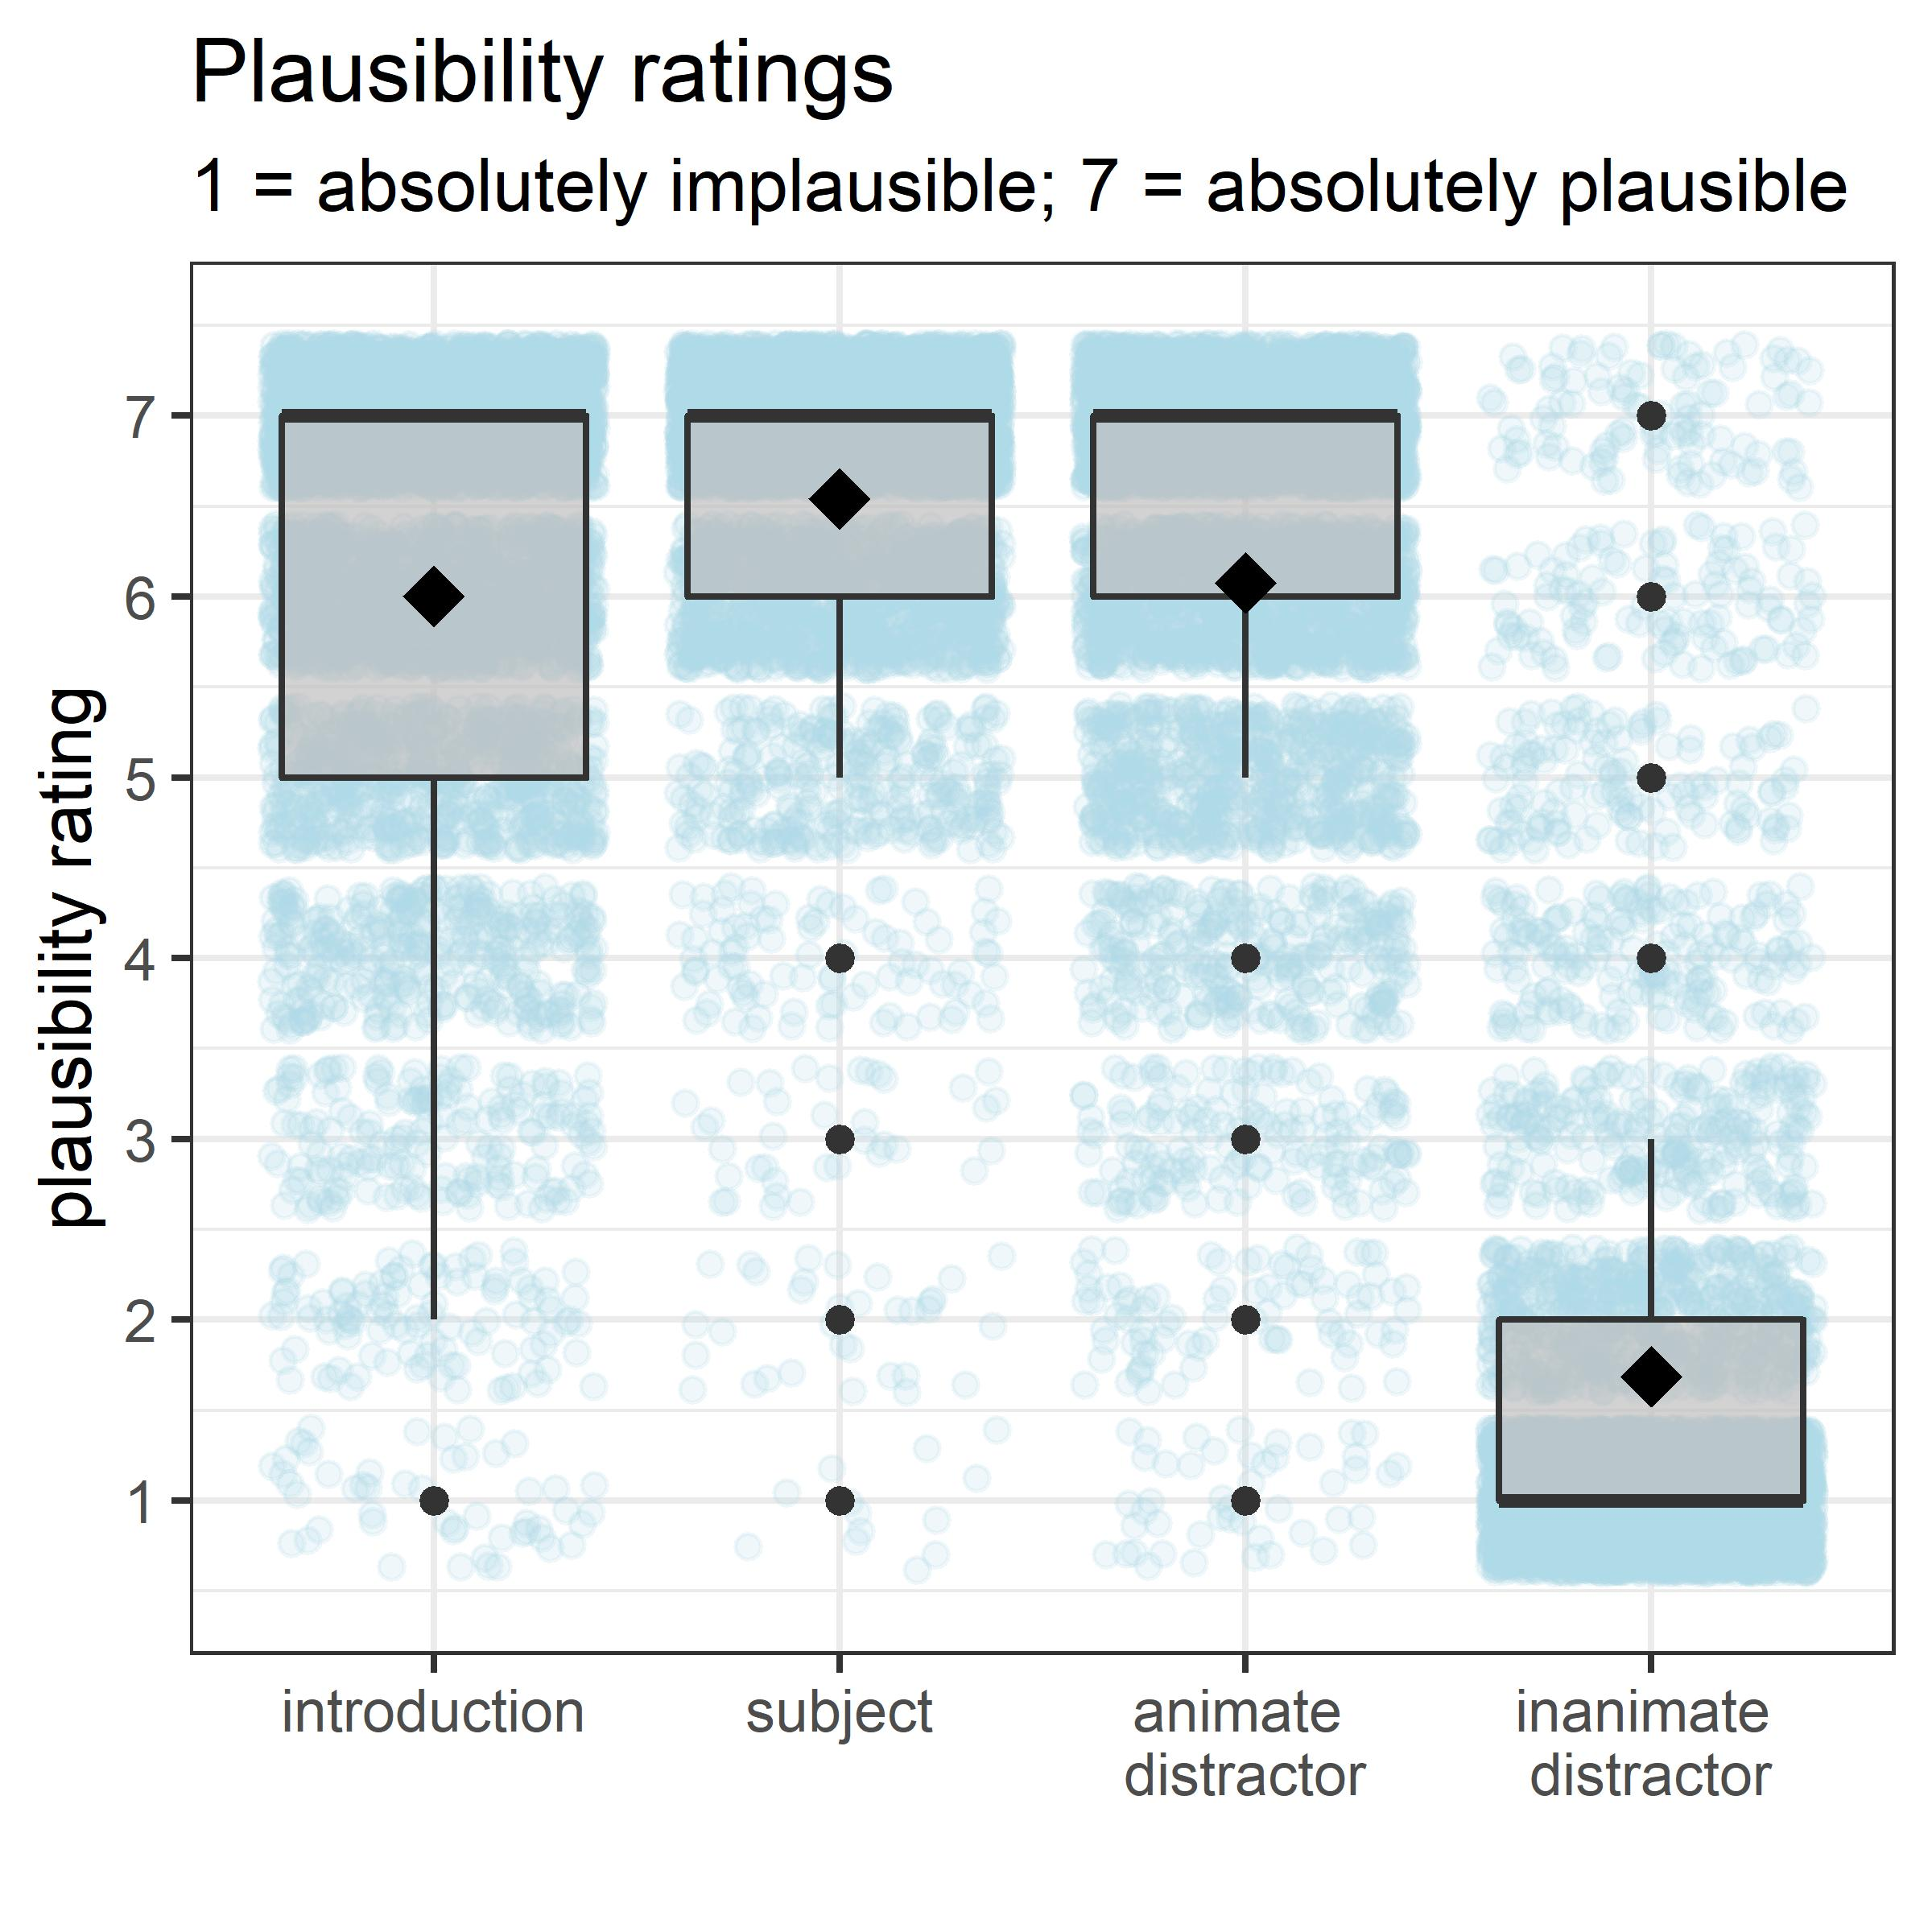
\includegraphics[width=0.6\textwidth]{images/pandora_plausibility_ratings.jpg}
\end{figure}


\subsection{The structure and sample sizes of the SPR and EEG experiments}

The SPR experiments were conducted web-based via Prolific and the EEG experiment was of course run in the lab.  Because the high signal-to-noise ratio of EEG data requires a large number of trials per condition and participant, we constructed 120 items. In order to keep the SPR and EEG studies comparable, we also used 120 items in the SPR experiments. In both methods, as it would have been very taxing for the participants to read all 120 items in one experimental session, we split the experiments into two sessions. 

The SPR study, hereafter Experiment 1a, was initially designed so that participants  (N=160) read items in the first session (1-60) and then, after a gap of 1-20 days, they read the the second set of items (61-120). The variation between participants in the gap is due to the fact that we could not control when the participants would do the second session; however, the mean and median gaps were  about 11 days, with the first and third quartiles being 9 and 12 days.

As discussed in detail below, the second session showed an adaptation effect \parencite{prasad2021rapid}: the effects observed in the first session disappeared. The adaptation effect is theoretically interesting per se \parencite{fine2013rapid} and we discuss it below; but it was problematic for our design because the average effect would then be confounded by adaptation. For this reason, we ran a second version of the SPR study, hereafter Experiment 1b, in which participants (N=614) were either shown items 1-60 or items 61-120 (but not both). In the Results section, we present both sets of results as well as the pooled data (N=774) from E1a and E1b.
As mentioned above, because the ERP method requires a large number of items, all the ERP data come from participants who completed both sessions. 

Figure \ref{fig:project_str} shows the structure of the present study, i.e., how many participants saw which subset of the items and whether these participants completed one or two experimental sessions.

\begin{figure}[H]
    \caption{The structure of the present study. In total, 120 items were used for the SPR (red branches) and the ERP experiments (blue branches). The color brightness reflects how many sessions were completed by each participant (lighter color: two sessions, darker color: one session).}
    \label{fig:project_str}
    \centering
    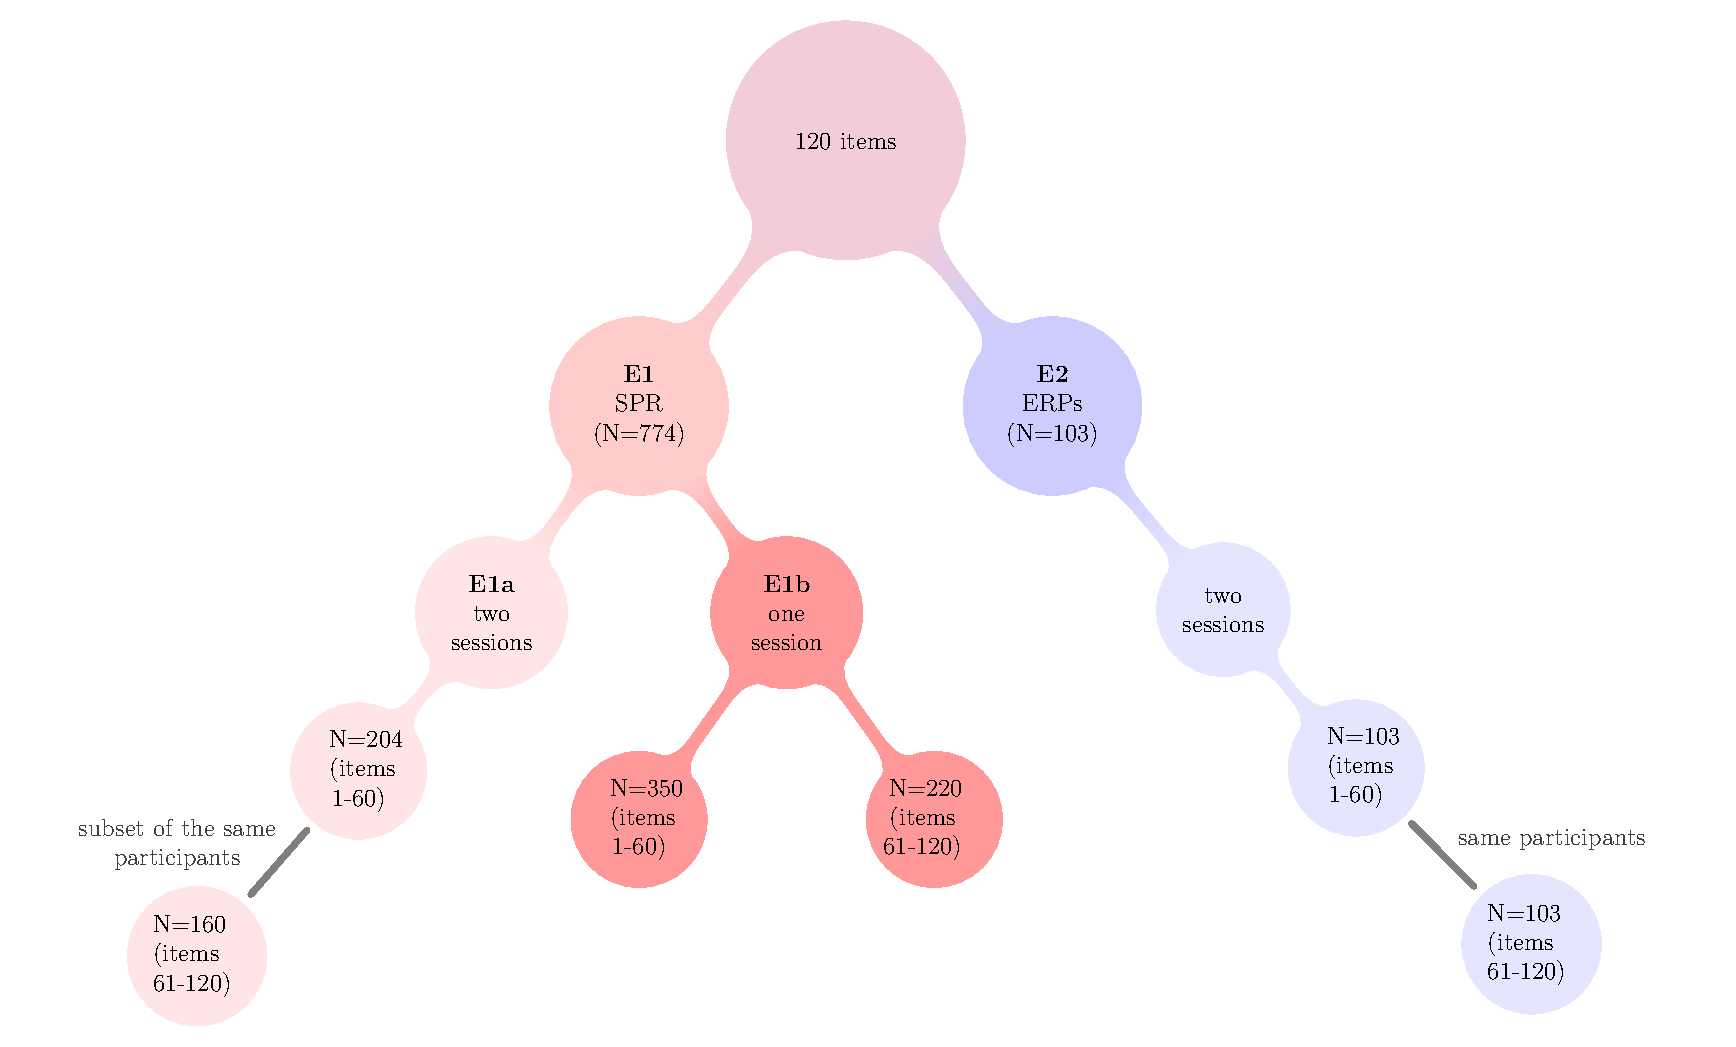
\includegraphics[width=0.85\textwidth]{images/pandora_project_structure_figure.pdf}
\end{figure}


\section{Experiments 1a and 1b: SPR}
%\subsection{Methods}

%Initially, we planned to conduct SPR experiment in two sessions to gain data from all participants for all 120 items. Collecting data for 120 items in one session was not considered feasible in a web-based SPR experiment, as the experiment duration would have been close to one hour. So, the first batch of participants (160 out of 774) completed two experimental sessions. This approach was dropped after we realized, that participants adapted to the task quickly which led to a considerable reading time speed-up between sessions (see Figure \ref{fig:whole_sentence} D). After this realization, all further participants took part in a single session during which they read half of the 120 items (for a visualization of the project structure, see Figure \ref{fig:project_str}).


\subsubsection{Participants}
%two sessions, session 1
% 224 participants completed
% 17 low acc
% 2 inconsistent demographic info
% 1 technical error
% final 204

% two sessions, session 2
% 178 participants completed
% 18 low acc
% final 160

% rep s1
% 387 participants completed
% 31 low acc
% 6 inconsistent demographic info
% final 350 

% rep s2
% 279 participants completed
% 51 low acc
% 8 inconsistent demographic info
% final 220

% 224 + 18  + 387 + 279 = 908

Native German-speaking participants were recruited via Prolific. In total, 908 participants took part in the self-paced reading experiments E1a and E1b. 117 participants were excluded due to low comprehension question accuracy (< 70\,\%). Additionally, 16 participants were excluded because the demographic information in their Prolific profile and the information which they provided during the experiment did not match (regarding, e.g., their native language, language impairment, or age). One participant was excluded because of a technical error during their session. The data of 774 participants (mean age: 27 years old, age range: 18 - 40 years, 395 female, 369 male, 10 preferred to not provide sex information) were used for analyses. When asked about their highest level of education, 365 participants reported a bachelor's degree or higher university education. 334 participants reported to have a high-school diploma and 70 another secondary school certificate. Five participants replied with ``other.'' 
%We conclude that the participants who were recruited via Prolific were slightly older and have a comparable or higher level of education than the typical undergraduate and graduate students who participate in lab-based studies.

In Experiment 1a, drop-outs between sessions led to a lower sample size in the second session (204 vs.\ 160). In Experiment 1a, compensation for the first session was \pounds 3.5 and for the second session, it was \pounds 5. In Experiment 1b, compensation was \pounds 4. 

\subsubsection{Procedure}
Participants completed a moving window self-paced reading task \citep{just_etal_1982} on the PCIbex Farm \citep{pcibex}. They were instructed to read for comprehension at a comfortable pace. All sentences were displayed word by word. Masked words were presented as a line indicating its length. Unmasked words were presented in 18 pt Courier font. The space bar on the keyboard was used to unmask words. The length of the sentences required line breaks. These were hard-coded so that in each sentence a line break appeared i) between the subject and the relative clause and ii) two words after the critical verb (see \ref{ex:linebreak}, critical word in bold, | indicate line breaks in the moving window display). In a third of the trials, the sentence was followed by a yes/no comprehension question. The participants received no feedback on their performance.

In addition to the reading-for-comprehension task, the participants completed two types of attention and compliance checks. The attention checks required them to press one of two designated keyboard keys ten times during each session. The compliance checks required them to type in two types of fruit and two hobbies (session 1) and two German cities and two breakfast food items (session 2). No participant failed any of these checks. The reader can try the experiment via this link \hyperlink{https://farm.pcibex.net/r/CBkSKl/}{https://farm.pcibex.net/r/CBkSKl/}. 

\begin{exe}  
\ex \label{ex:linebreak}
    \gll Die Nachbarin glaubte, dass der Witwer, | der erzählt hatte, dass der Verlust schrecklich war, regelmäßig abends \textbf{trank}, um zu | vergessen. \\ 
    The neighbor believed that the widower | who told had that the loss awful was regularly in.the.evening drank in.order to | forget\\
    \trans  `The neighbor believed that the widower, who had told her that the loss was awful, regularly drank in the evenings to forget.'\\  
\end{exe}

In Experiment 1a, participants were re-invited for session 2 after they completed session 1. The experimental sessions were separated by 1 - 20 days. The procedure of the sessions was identical. Each session lasted approximately 25 minutes.

\subsubsection{Statistical analyses}

\paragraph{Bayesian linear mixed models}
Comprehension question accuracy was analyzed with Bayesian generalized linear mixed models, i.e., logistic regression, in R \citep{r}, using the brms package \citep{brms}. The fixed effects were syntactic interference, semantic interference and their interaction. These were sum-contrast coded (high +0.5, low -0.5). Varying intercepts for participants and items were included. For the intercept, we used a Normal(0, 1.5) prior and  for all fixed-effect slope parameters, a Normal(0, 0.1) prior. The priors for the variance components were the defaults specified in brms. Models were run with 4 chains and 8,000 iterations in each chain. 2,000 iterations in each chain consisted of a warm-up phase. 

Self-paced reading times were analyzed with Bayesian linear mixed models in R \citep{r} with log-normal likelihood, using the brms package \citep{brms}. The critical word for analyses was the verb \textit{trank} `drank' in \ref{ex:materials}, constituting the retrieval site. Because previous work found effects in the pre-critical and post-critical region, reading times of the pre-critical word (\textit{regelmäßig} `regularly' in \ref{ex:materials}) and the spill-over region (\textit{um} `in.order.to' in \ref{ex:materials}) were analyzed. 
The models included fixed effects for syntactic interference (high +0.5, low -0.5), semantic interference (high +0.5, low -0.5) and their interaction.  Varying intercepts for participants and items were included; varying slopes were excluded for reasons explained below. 

\paragraph{Bayes factors for model comparison}

In order to quantify the uncertainty on the parameters of interest, we report 95\% credible intervals.  
These intervals represent the range over which we can be 95\% certain that the values of the parameter lies, given the statistical model and the data. However, formal hypothesis testing cannot be carried out without a likelihood ratio test that compares two alternative models \parencite{schad_etal_2022_BF,Royall}. For this reason, formal hypothesis tests for the presence or absence of the effects of interest were carried out using Bayes factors. Because Bayes factors can be very sensitive to prior specifications on the target parameter being tested \parencite{schad_etal_2022_BF}, 
we report a sensitivity analysis using a range of prior specifications for the relevant parameters (see Table \ref{tab:spr_priors}). The priors assume a priori effect sizes for the main effects of syntactic and semantic interference, and their interaction, ranging from 0-8 ms, 0-40 ms, or 0-81 ms.  These priors are based on the observed effect sizes and their uncertainties in previous reading studies that use the present design \parencite{vandyke07,mertzen}.

The Bayes factor is analogous to the frequentist ANOVA or likelihood ratio test: it compares the (marginal) likelihood of a full model to that of a baseline null model; this is often written as $BF_{10}$, with the subscripts indicating that marginal likelihood of the full model is in the numerator and that of the null model is in the denominator. One major advantage of the Bayes factor over the frequentist analogue is that it takes the uncertainty of the parameters into account. This leads to more conservative inferences compared to frequentist ANOVA, which only takes the maximum likelihood estimate of the parameter into account \parencite[see][for detailed discussion]{schad_etal_2022_BF}. Another important advantage of the Bayes factor -- one that is very relevant for the present work -- is that it is in principle possible to find evidence both for or against an effect. This stands in contrast to the frequentist ANOVA, which is designed to only furnish evidence against the null. 

Bayes factors can be interpreted as follows \parencite[e.g., ][]{lee2014bayesian}: if BF$_{10}$ > 1, it provides evidence in favor of the effect of interest. If BF$_{10}$ < 1, it provides evidence in favor of the null model. The larger the value of BF$_{10}$, the stronger the evidence for the effect and the smaller the value of BF$_{10}$ is, the stronger the evidence for the null. 
In general, a large number of iterations is needed in the brms package in order to obtain stable estimates of the Bayes factor  \citep{schad_etal_2022_BF}.
For this reason, models were run with four chains and 20,000 iterations in each chain, with the first 2,000 iterations in each chain being discarded as the warm-up phase.  Bayes factors were unstable when varying slopes were included; for this reason, we fit the models only with varying intercepts by participant and by item.

\begin{table}[h]
    \caption{Priors used for the analysis of the self-paced reading time data. Priors on the fixed-effects slope parameters were truncated to a lower bound of zero, i.e., only positive values were assumed to be possible a priori. This corresponds to the existing evidence in the literature that high interference conditions lead to longer reading times than low interference conditions. The standard deviation of the fixed-effects slope priors was varied in order to conduct a Bayes factor sensitivity analysis following \citet{schad_etal_2022_BF}. See the corresponding assumed a priori range of the difference between reading times under high vs.\ low interference on the millisecond scale.}
    \label{tab:spr_priors}
    \centering
     \begin{tabular}{lllr}
    \toprule
    Parameter&Prior & &Assumed Range in ms\\
    \midrule
  Intercept & Normal(6, 0.6)& & [125, 1308]\\
  \cmidrule{2-4}
  \multirow{3}{1cm}{slope} & Normal(0, 0.01) & \hspace{-1em}\rdelim\}{3}{*}[lower bound: 0] & [0, 8]\\
  &  Normal(0, 0.05)& & [0, 40]\\
  & Normal(0, 0.1) & &[ 0, 81]\\
  \cmidrule{2-4}
  sigma & Normal(0, 0.5)&  \hspace{-1em}\rdelim\}{2}{*}[lower bound: 0]&\\
  SD & Normal(0, 0.1)& &\\
  \bottomrule
  \end{tabular}
  \end{table}
 
%\bigskip

%\begin{table}[ht]
%    \centering
%        \caption{Contrast coding.}
%    \label{tab:contrasts}
%    \begin{tabular}{cccc}
%\toprule
%condition & syntactic interference & semantic interference & interaction\\
%\midrule
%a)  LoSyn LoSem &  $-1$& $-1$ & $+1$ \\
%b)  LoSyn HiSem & $-1$ & $+1$ & $-1$  \\
%c)  HiSyn LoSem &  $+1$ &$-1$ & $-1$    \\ 
%d)  HiSyn HiSem &  $+1$ &$+1$  & $+1$   \\
%\bottomrule
%    \end{tabular}
%\end{table}


\subsubsection{Comprehension question accuracy (Experiments 1a and 1b combined)}

After exclusion of participants with accuracy below 70\,\%, overall accuracy (including fillers) was good; on average 85.9\,\% (range: 71.9 - 100\,\%). Accuracy for the critical items was 81.1\,\% (range: 20 - 100\,\%). Condition-wise accuracy is shown in Table \ref{tab:spr_acc}.

\begin{table}[]
    \caption{By-condition accuracy in critical trials in the SPR experiment (E1a and E1b combined).}
    \label{tab:spr_acc}
    \centering
    \begin{tabular}{llr}
    \toprule
    syntactic & semantic & accuracy \%\\
    \midrule
        low &  low & 86.0\\
        low &  high & 77.7\\
        high &  low & 85.8\\
        high &  high & 74.9\\
    \bottomrule
    \end{tabular}
\end{table}

Table \ref{tab:spr_acc_mod} shows the results of the generalized mixed model (log-odds scale) analyzing the comprehension accuracy for the critical items (Experiments 1a and 1b combined). The estimates and 95\,\% credible intervals show primarily a reduction in comprehension accuracy for high compared to low semantic interference conditions.

\begin{table}[H]
    \caption{Results in log-odds from the Bayesian generalized model analyzing the comprehension accuracy in the SPR Experiments 1a and 1b.}
    \label{tab:spr_acc_mod}
    \centering
    \begin{tabular}{lrr}
    \toprule
    & Estimate &  95\% CrI  \\
    \midrule
Intercept& 1.66 &   [1.38, 1.93]\\
syntactic& -0.08 &  [-0.16, -0.01]\\
semantic&  -0.61 & [-0.69, -0.54]\\
interaction& -0.10&  [-0.22, 0.02]\\
    \bottomrule
    \end{tabular}
\end{table}

Since the accuracies are not of primary interest, we do not carry out Bayes factors analyses for these.

\subsubsection{Self-paced reading times (Experiments 1a and 1b combined)}

\paragraph{Estimated effect sizes and their uncertainty}

Reading times across the whole sentence are shown in Figure \ref{fig:whole_sentence} A and B, separately for high and low syntactic interference because these conditions had partially different sentence structures. 

\begin{sidewaysfigure}[h]
    \caption{Self-paced reading times with 95\% confidence intervals. Panel A and B show the pooled reading times across the whole sentence; separately for high (A) and low (B) syntactic interference due to differing sentence structure. Panel C shows the pooled reading times of all conditions in the critical and surrounding regions. Panels D and E show the reading times of all conditions in the critical and surrounding regions in the different parts of the self-paced reading experiment.}
    \label{fig:whole_sentence}
    \centering
    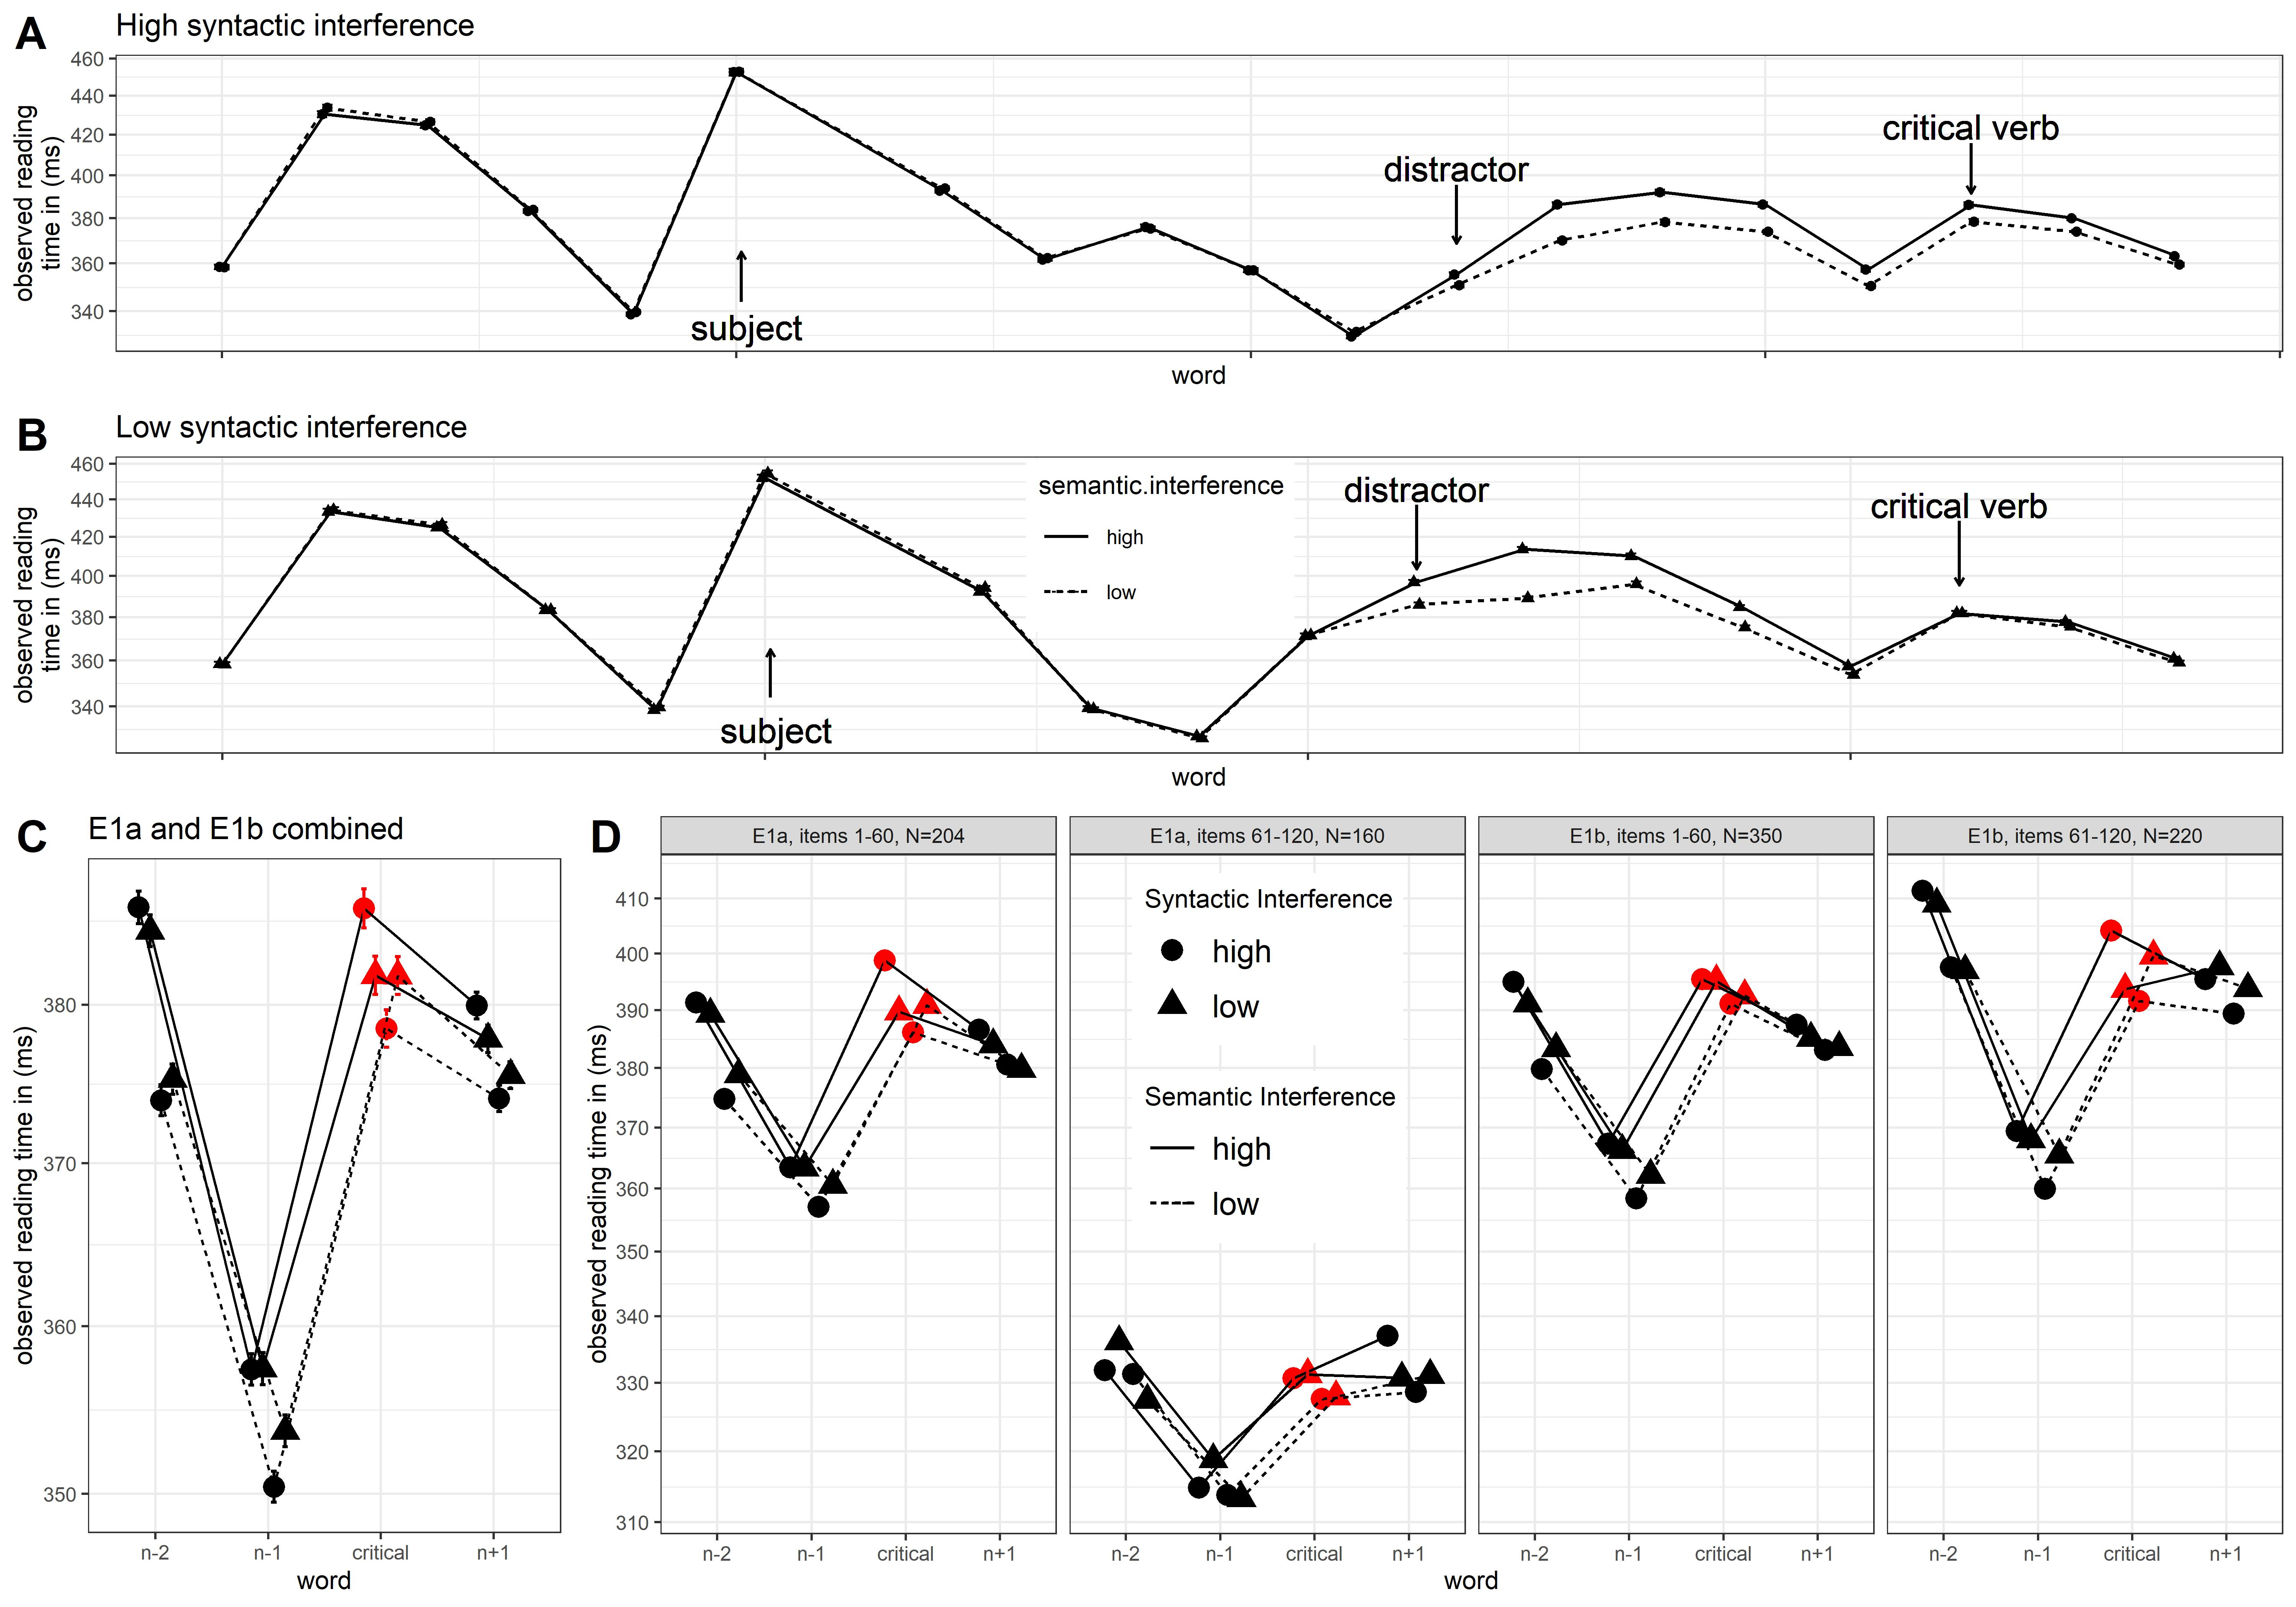
\includegraphics[width=0.85\textwidth]{images/Pandora_all_wholesentence_pooled_zoom_exp.jpg}
\end{sidewaysfigure}
\clearpage

It is apparent from Figure \ref{fig:whole_sentence} A and B that, regardless of the syntactic manipulation, at the distractor, reading times between high and low semantic interference started to differ: distractors in the high semantic interference conditions induced longer reading times than in the low semantic interference conditions. This pattern persisted in the following regions.

Because the distractor and the immediately following regions differ between conditions, we did not compute Bayes factors for the observed reading time differences. Instead we focused our Bayes factors analyses on regions which were identical across conditions. These are the pre-critical, critical and spill-over regions.

%This is probably due to encoding interference \citep{mertzen, jaeger_etal_2015_retrieval_encoding} and persisted in the following regions.  

Figure \ref{fig:whole_sentence} C shows the reading times of these regions; here, we also show the pre-pre-critical region, which was identical across conditions as well, but will be harder to interpret because of possible spill-over from the syntactic manipulation. The pre-pre-critical and pre-critical region show longer reading times for high vs.\ low semantic interference conditions. The critical verb was read slowest when syntactic and semantic interference were both high and fastest when syntactic interference was high and semantic interference low. The other two conditions showed intermediate reading times. The spill-over region again primarily showed a difference between high and low semantic interference conditions. 

Panels D and E show the reading times of the critical and surrounding regions for each of the two Experiments 1a and 1b. In Experiment 1a, the first session (items 1-60, N = 204, left sub-figure) showed results similar to the pooled results presented in Panel C. In the second session of Experiment 1a (items 61-120, N = 160, right sub-figure) a smaller semantic interference effect was seen at the critical verb and the patterns in the surrounding regions were less clear than in the first session. Additionally, the second session in Experiment 1b showed shorter reading times compared to the first session. As mentioned earlier, this attenuation in reading times and differences between conditions is likely due to  adaptation to the task in the second session. 

Panel E shows that Experiment 1b with items 1-60 (N = 350, left sub-figure) showed a pattern consistent with semantic interference in all regions. Experiment 1b with items 61-120 (N = 220, right sub-figure) showed a pattern consistent with semantic interference in the regions surrounding the critical verb, but not at the verb itself. At the verb, reading times were longest when both syntactic and semantic interference were high. Reading times were a bit faster when both syntactic and semantic interference were low. The other two conditions (high syntactic/low semantic and low syntactic/high semantic) lead to the fastest verb reading times in Experiment 1b with items 61-120. 

%These somewhat inconsistent results, especially in the critical region, across the sub-experiments and the random assignment of participants to the sub-experiments motivated us to gain estimates of the effects under investigation for the individual participants (see Figure \ref{fig:spr_individual}).

%\begin{figure}[H]
 %   \caption{Individual estimates of syntactic and semantic interference and their interaction at the critical verb for all 774 participants in the self-paced reading experiment. Shown are shrunken estimates from a Bayesian hierarchical linear mixed model. Circles show individual’s mean effects, errors bars are 95\,\% credible intervals. The red dashed line shows an effect of zero (difference of zero milliseconds). Two solid red lines mark an effect size of 10 and 20 ms, respectively.}
%    \label{fig:spr_individual}
 %   \centering
  %  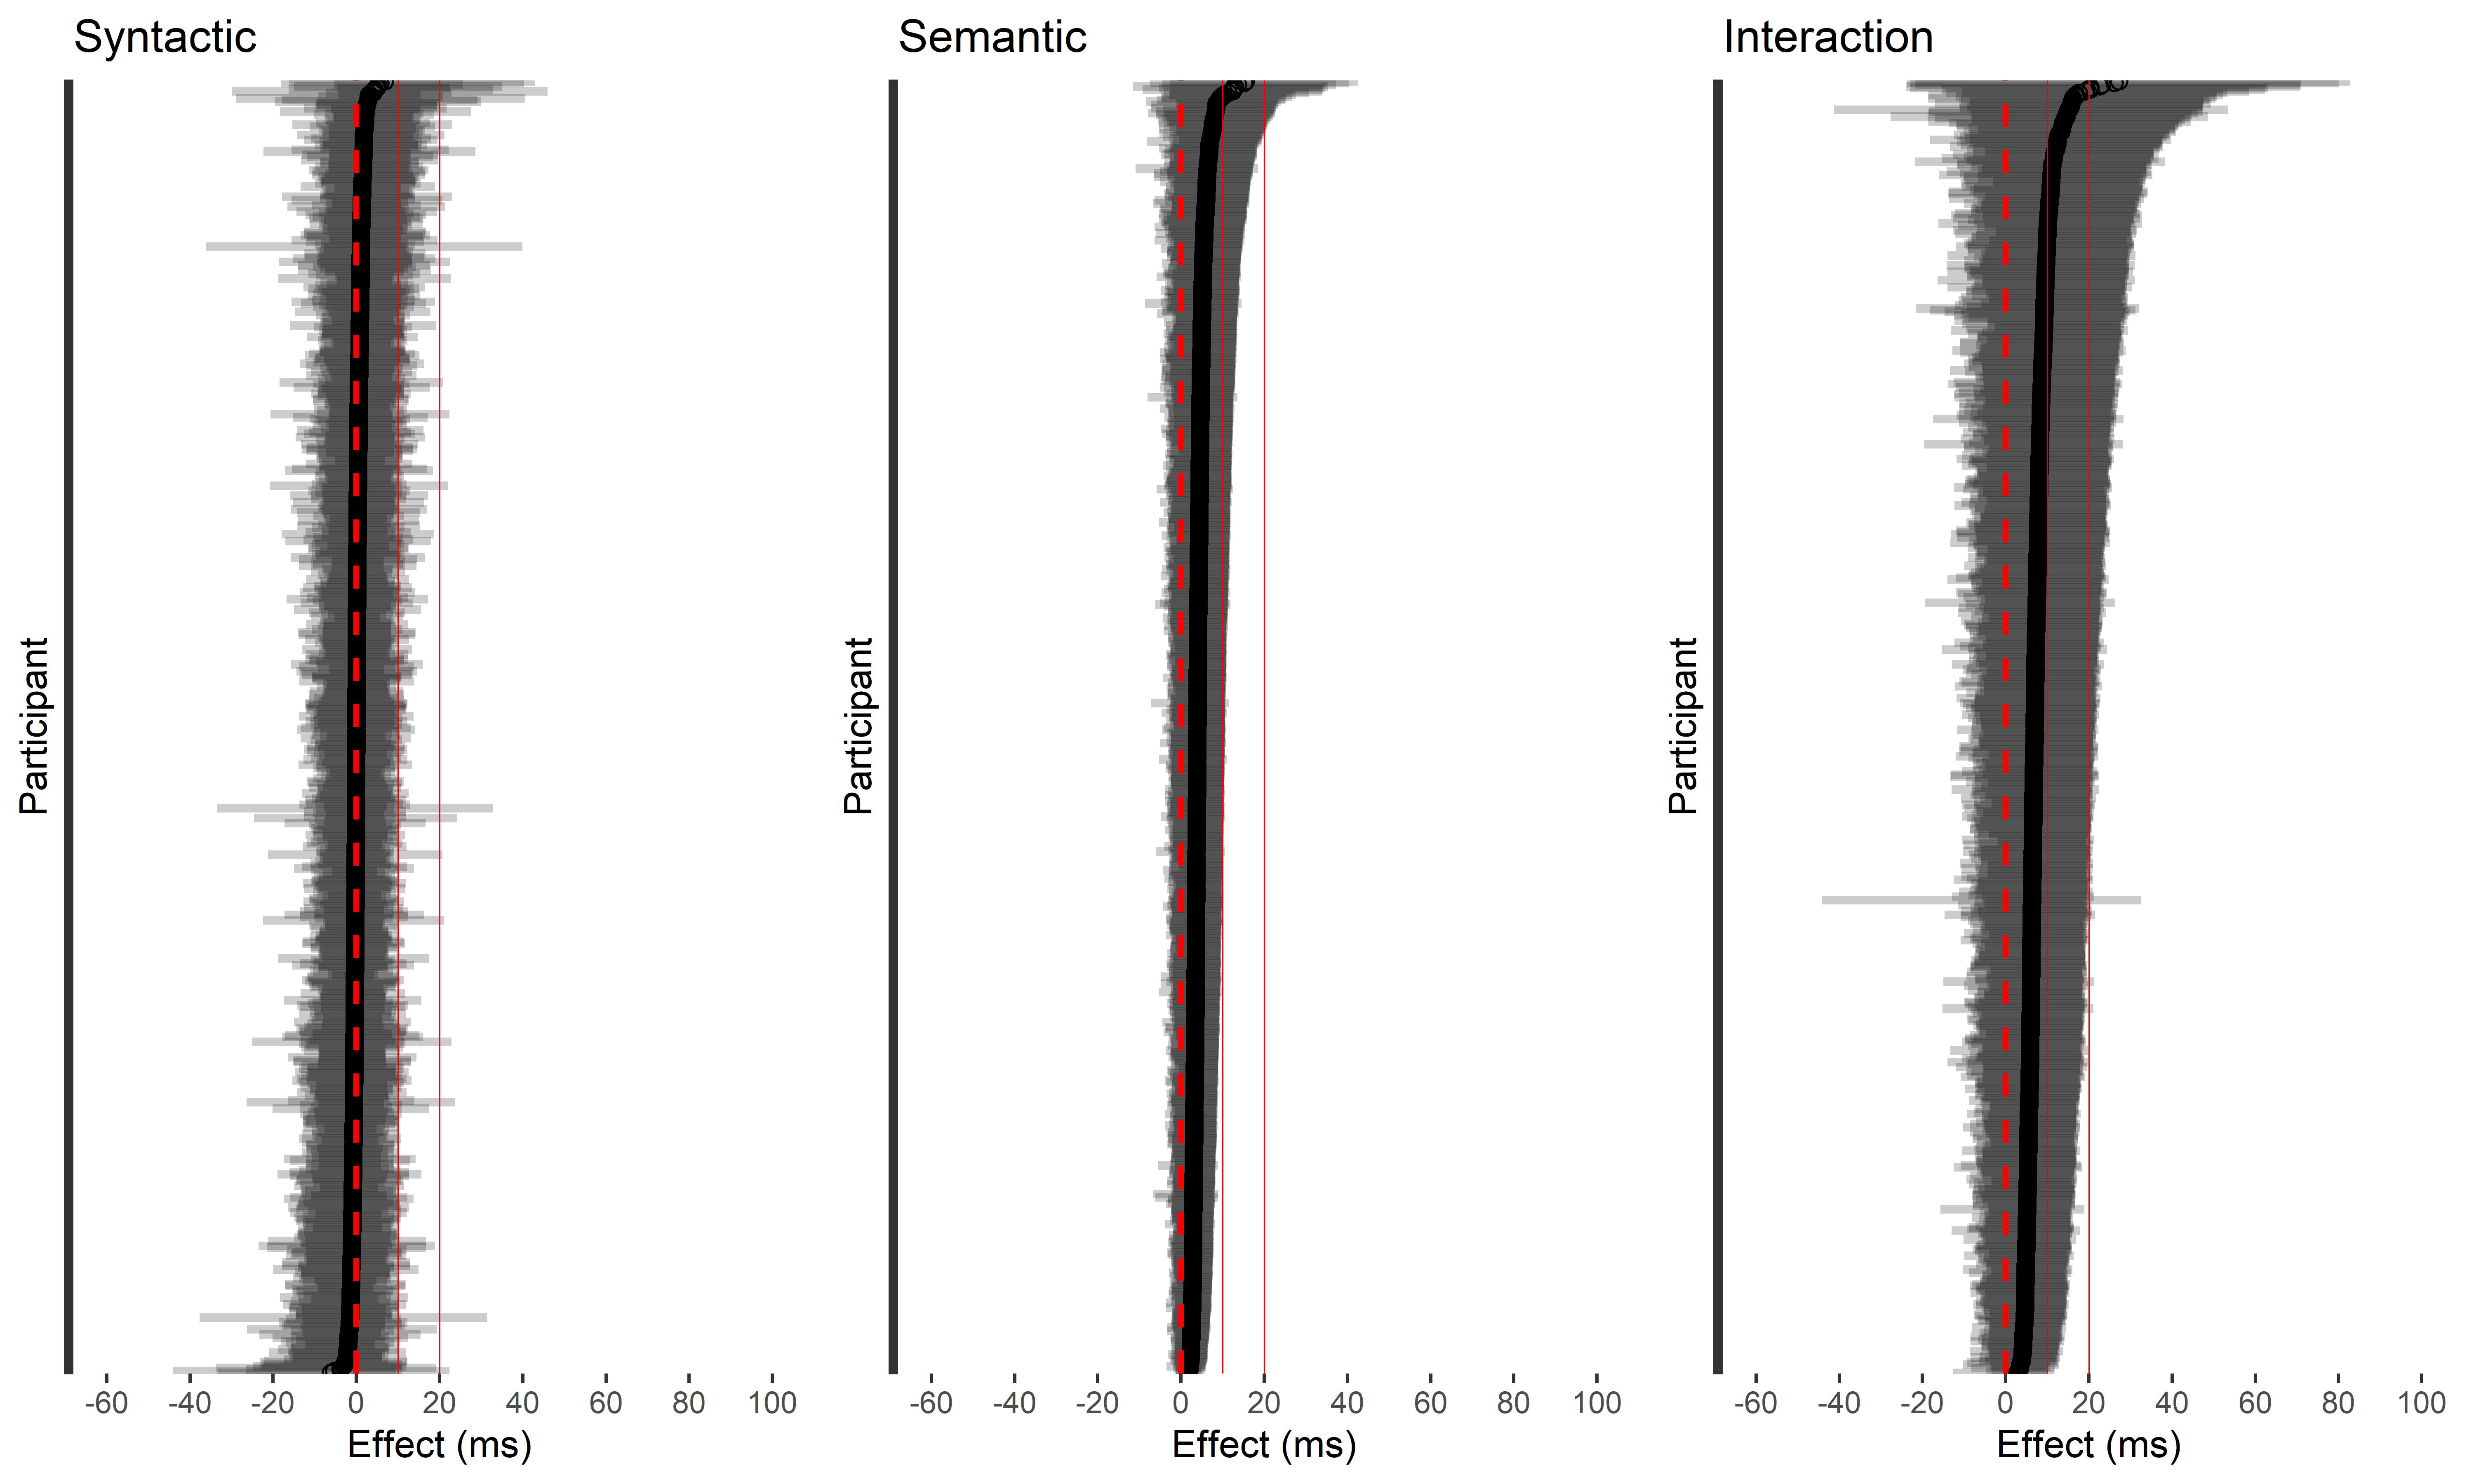
\includegraphics[width=\textwidth]{images/individual_diffs.jpg}
%\end{figure}

%The individual-level effects were derived from a Bayesian linear mixed model with the priors shown in Table \ref{tab:spr_priors} with the intermediate slope prior of Normal(0, 0.05) and random slopes for syntactic and semantic interference and their interaction but without correlations of random effects.


%Figure \ref{fig:spr_individual} shows that at the critical verb, the 95\,\% credible intervals for the syntactic interference effect of all participants were centered around zero. In contrast, participants consistently displayed a small effect of semantic interference with narrow 95\,\% credible intervals. The individual-level estimates of the interaction were a bit larger but they were associated with more uncertainty (wider 95\,\% credible intervals). The individual-level results help to understand the population-level posteriors presented in Figure \ref{fig:spr_posteriors} and the population-level Bayes factor analysis (see Figure \ref{fig:spr_bfs}). 

Turning now to the estimates of the main effects and interaction parameters in the pooled data (Experiments 1a and 1b combined), Figure \ref{fig:spr_posteriors} shows that the pre-critical, critical and spill-over regions showed very similar posterior distributions for the parameters. For syntactic interference, they were close to zero in all regions. In contrast, for semantic interference, the estimates ranged between [8,14] ms (pre-critical), [4, 12] ms (critical), and [5, 11] ms (spill-over region). The posteriors for the interaction were consistent with an interaction effect. The interaction was the  largest in the critical region ([7, 22 ms]). 

\begin{figure}[H]
    \caption{Posteriors for the syntactic and semantic interference effects and their interaction at the critical verb and surrounding regions in the pooled self-paced reading data (Experiments 1a and 1b combined). The numerical values are the means and 95\,\% credible intervals. The blue vertical lines represent the median and the blue shaded areas are 80\,\% credible intervals.}
    \label{fig:spr_posteriors}
    \centering
    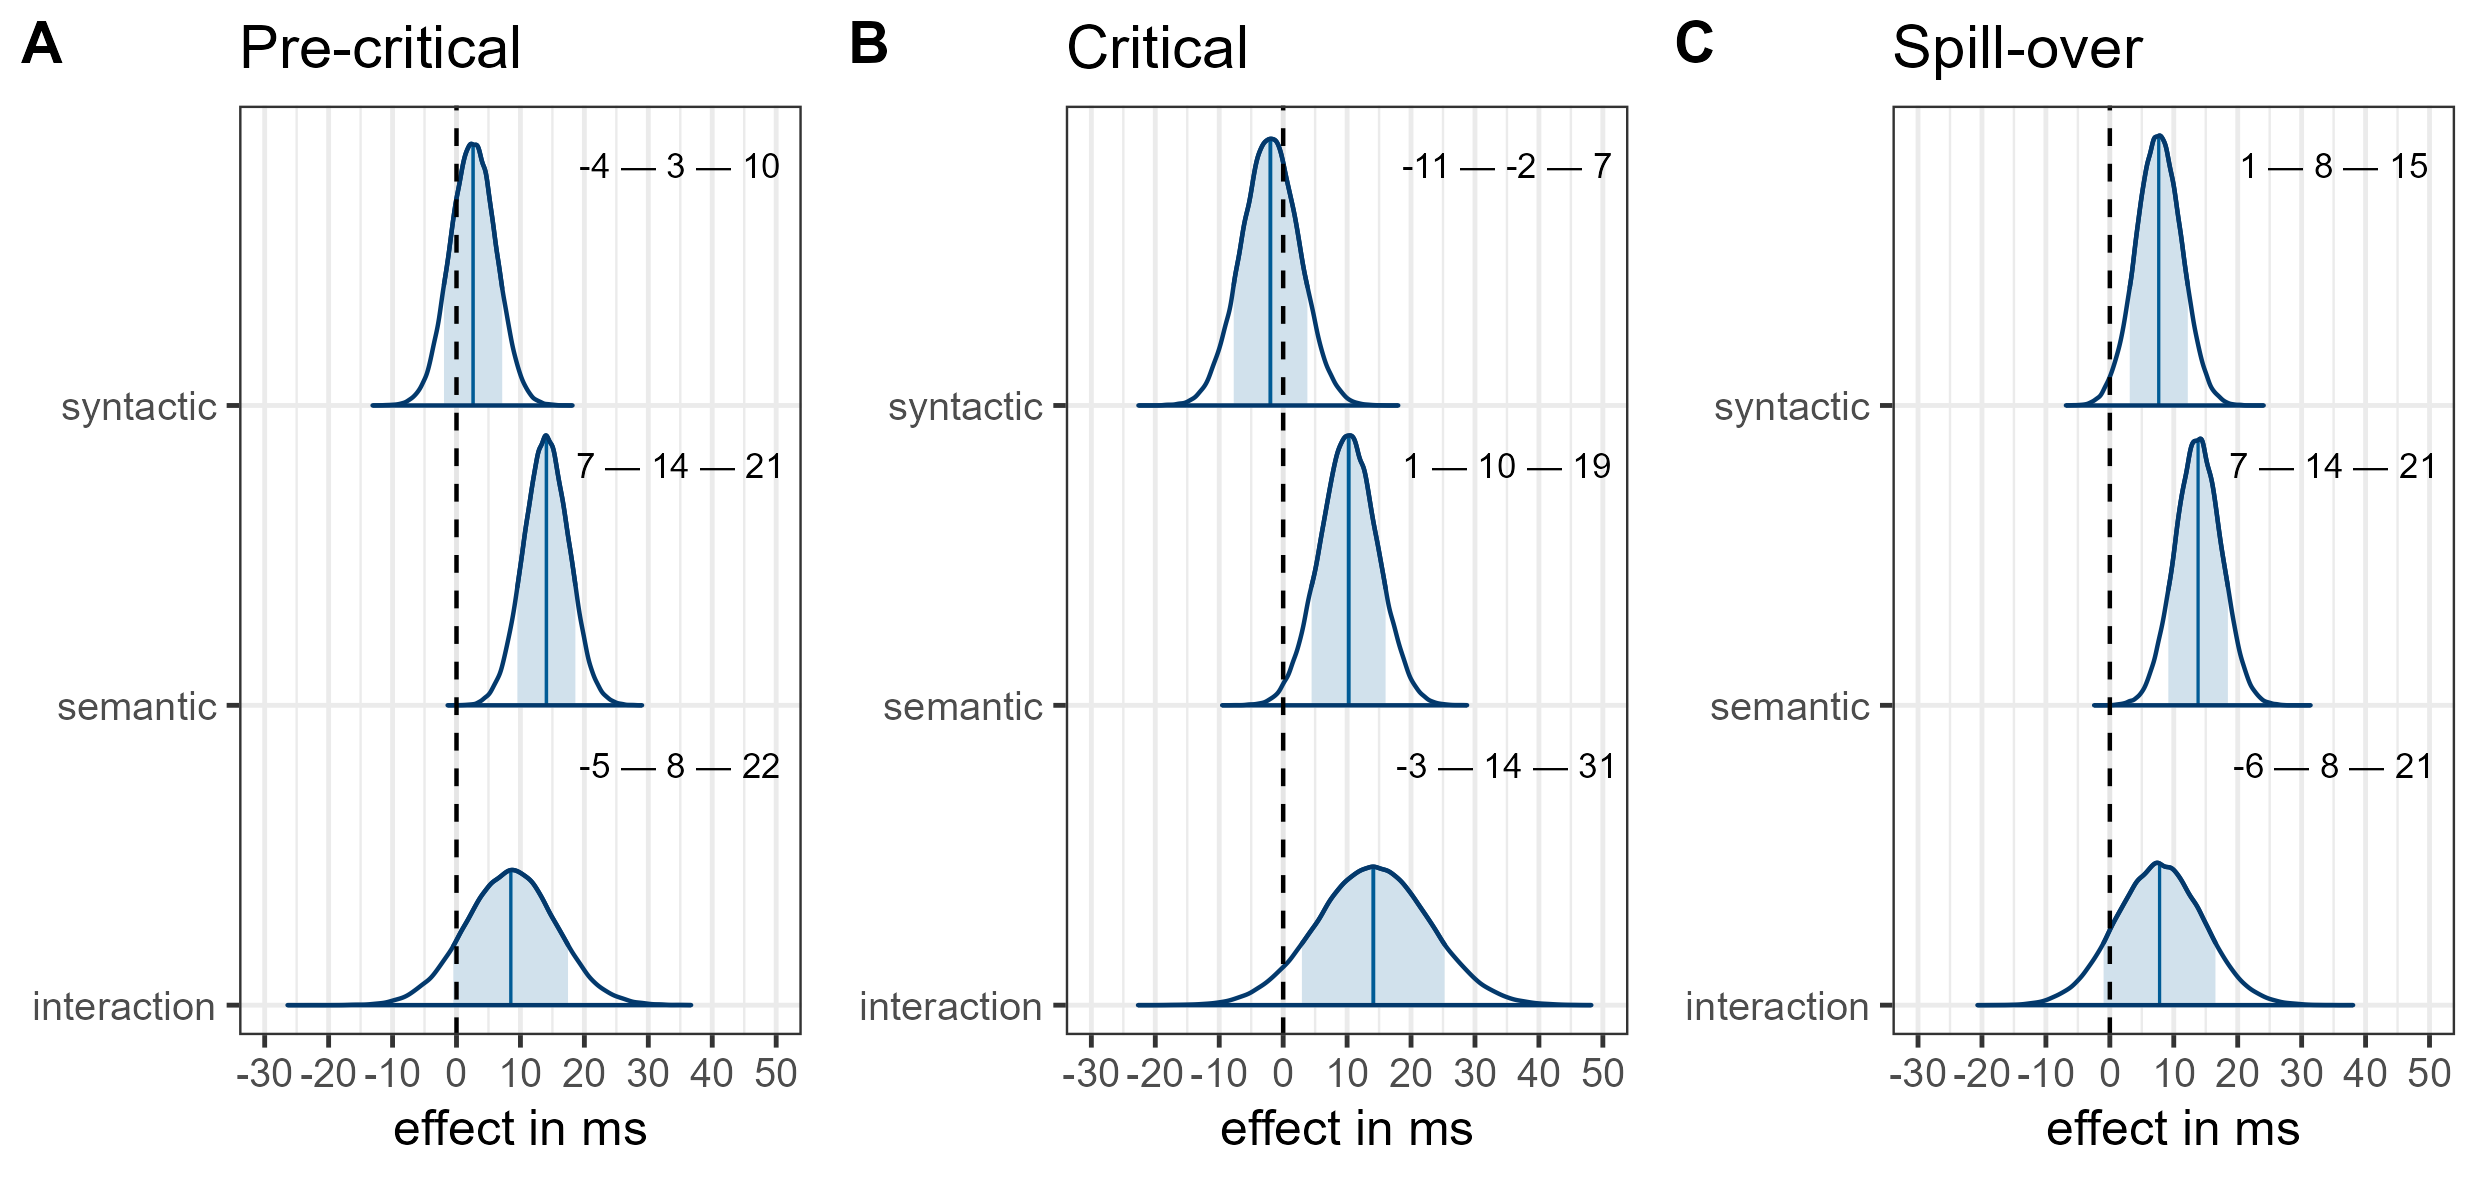
\includegraphics[width=\textwidth]{images/posteriors_spr_pooled_774.png}
\end{figure}

\paragraph{Hypothesis testing using Bayes factors}

Was there any evidence for the effects estimated above? The Bayes factor analysis is presented in Figure \ref{fig:spr_bfs}. The analyses use all the data from Experiments 1a and 1b. We found extremely strong evidence for the semantic interference effect in the pre-critical, critical and spill-over regions (BF$_{10}$ > 200). No evidence was found for syntactic interference in any of the investigated regions; in fact, there is strong evidence against the syntactic interference effect in all regions and under all the priors used (BF$_{10}$ < 1).  Evidence for the interaction was only found in the critical region. Here, the evidence for the interaction was strong (BF$_{10}$ = 40) when the prior on the parameter was N+(0, 0.01), i.e., a small a priori effect size ranging from  [0, 8] ms; the evidence for the interaction was much weaker (BF$_{10}$ = 1.8) when the prior was N+(0,0.1), i.e., a larger a priori effect size ranging from [0, 81] ms. In other words, only if we assume a priori that the effect size for the interaction is relatively small, then there is strong evidence for this effect.

\begin{figure}[H]
    \caption{Bayes Factors for the effects of semantic interference, syntactic interference and their interaction in the reading times (combined Experiments 1a and 1b) at the critical verb and surrounding regions, under a range of priors on the target parameters.}
    \label{fig:spr_bfs}
    \centering
    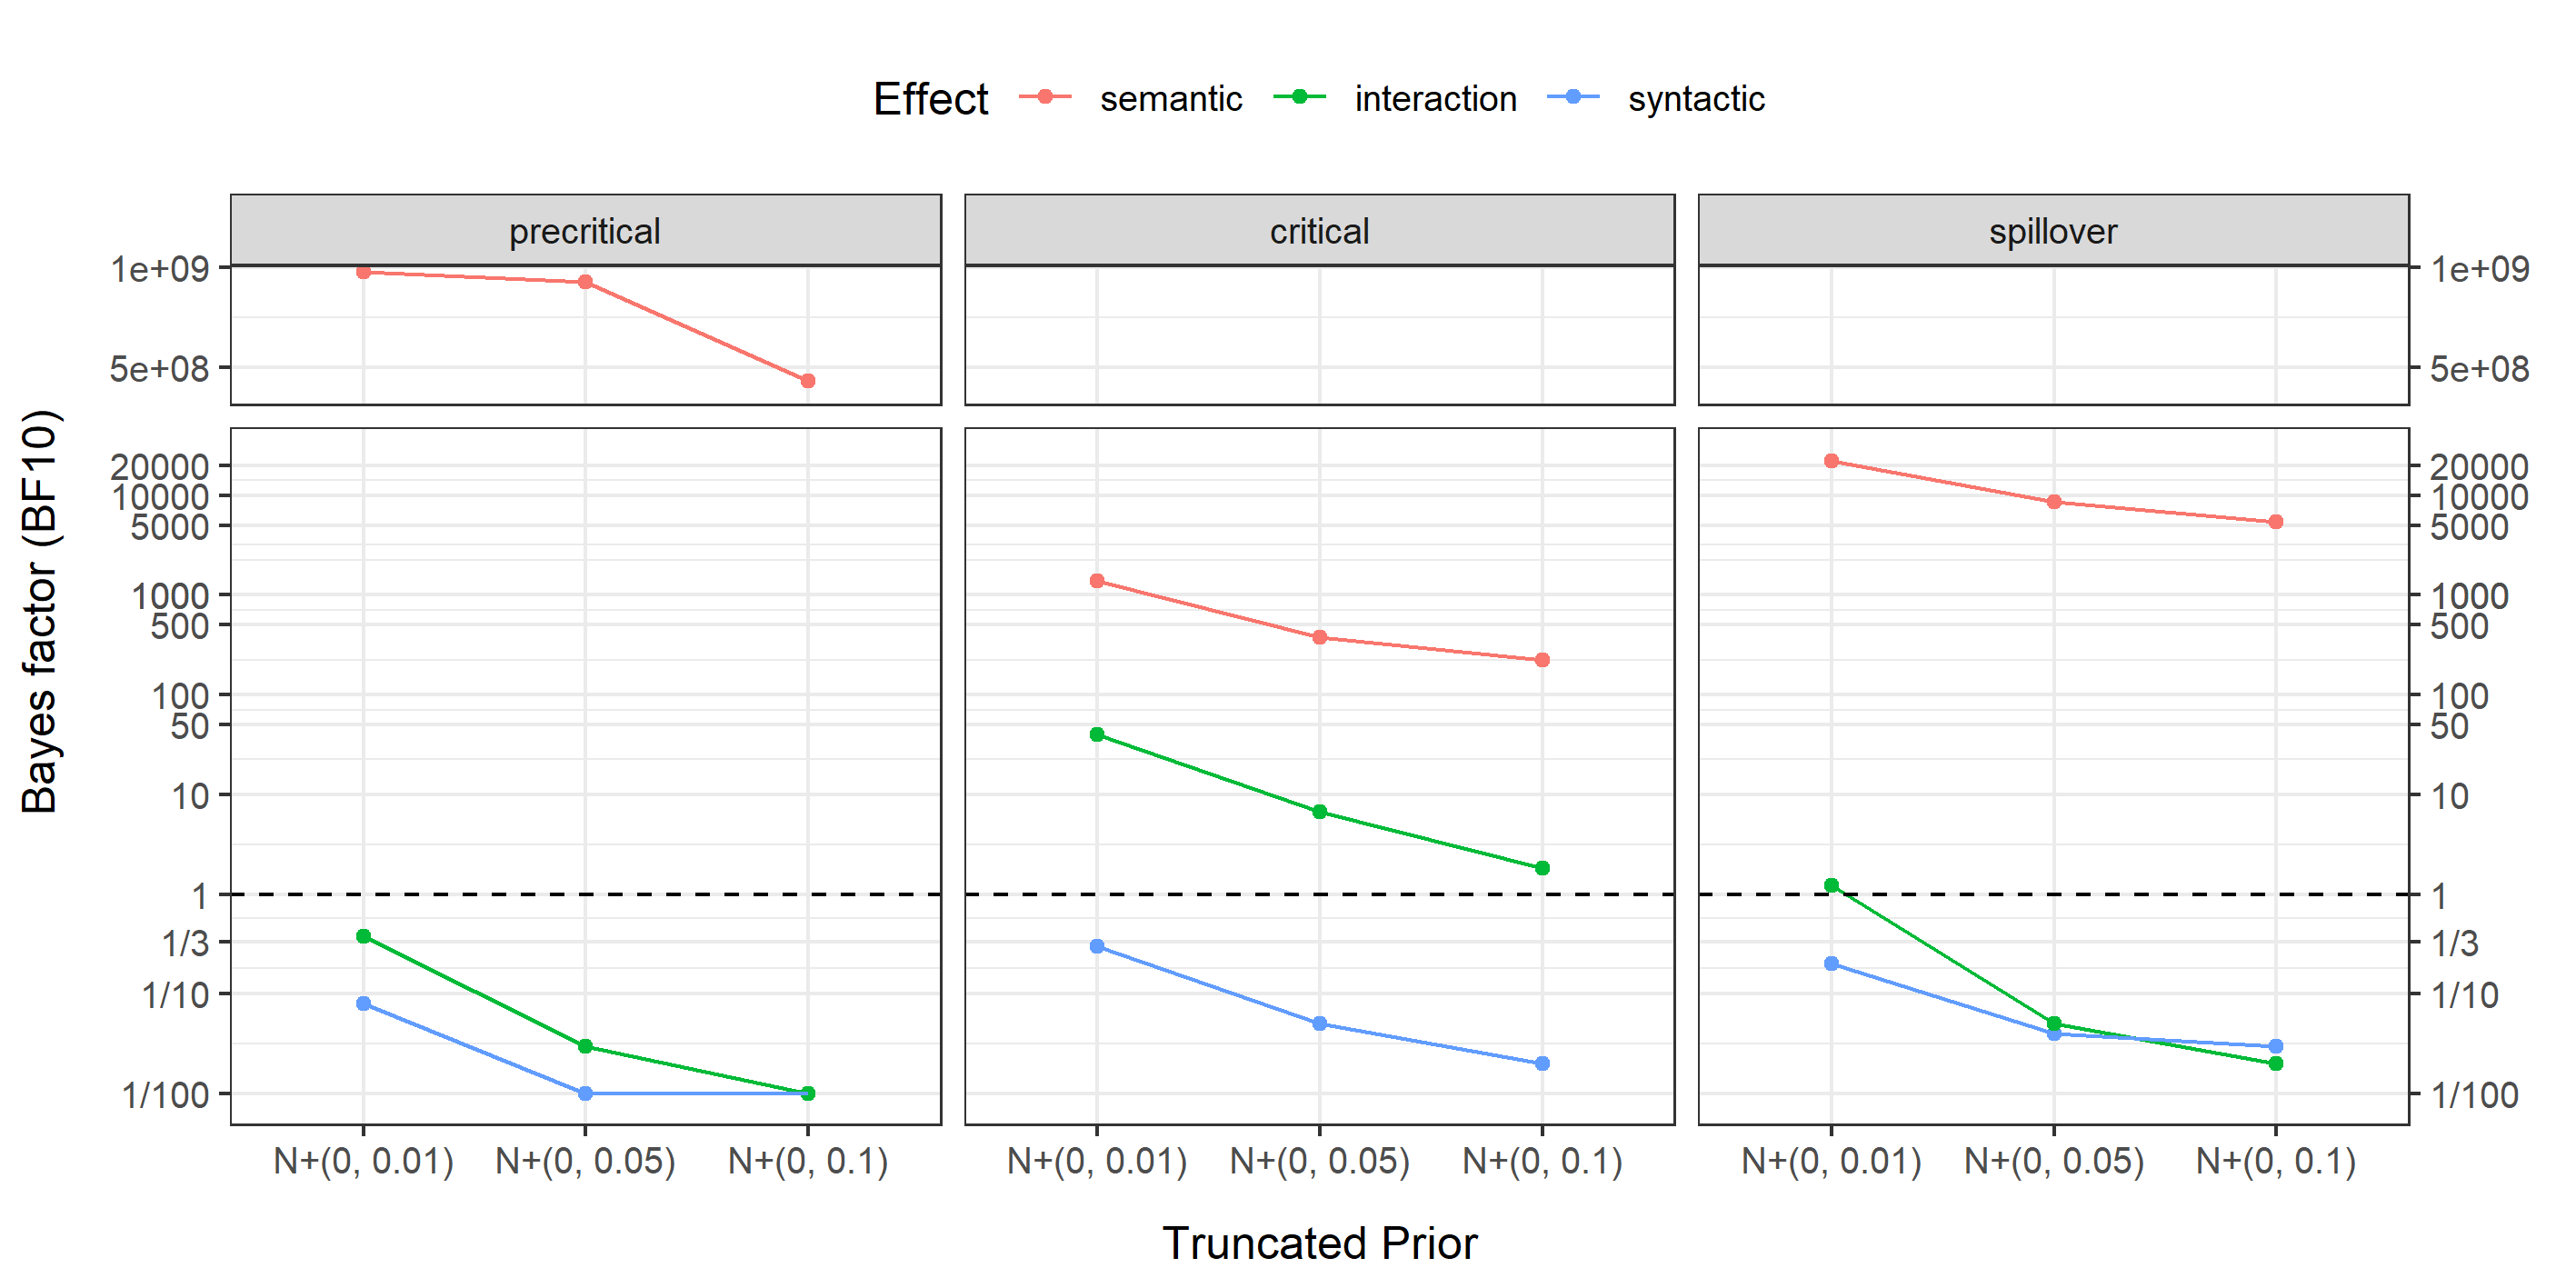
\includegraphics[width=\textwidth]{images/BF_plot_spr_774_allregions.png}
\end{figure}

\section{Discussion}
We presented a relatively large-sample self-paced reading study that investigated the use of syntactic and semantic features during subject-verb dependency formation. Reading times at the critical verb showed clear evidence for semantic interference, but evidence against syntactic interference. The semantic interference effect was already present at the pre-critical region; i.e., semantic interference occured even before the retrieval event could begin. 

\subsection{The effects in the pre-critical region}

At the distractor (which occurred well before the pre-critical region), high semantic interference (animate distractors) lead to longer reading times than low semantic interference (inanimate distractors, see Figure \ref{fig:whole_sentence} A and B). One might argue that this pattern could be due to differences in word length. The animate distractors in our materials were on average 1.1 letters longer than the inanimate distractors (mean length of animate distractors: 9.3, sd: 2.6, mean length of inanimate distractors: 8.2, sd: 2.9). It seems unlikely that this small difference in word length caused such large and long-lasting effects, but in order to be conservative we do not try to interpret this difference.

At the pre-critical region, there was clear evidence for semantic interference. As this cannot be due to retrieval interference, the most likely explanation is encoding interference \citep{Oberauer_Kliegl_2006}. The increased effort of encoding and subsequently maintaining representations of three different animate noun phrases (the introduction noun, the subject and the animate distractor) is the most likely reason for the slowdown in high vs.\ low semantic interference conditions \citep[for similar findings, see e.g., ][]{lago_etal_2021, kush_etal_2015, gordon02}. 

Indeed, previous work using the same design as in the present paper has also found semantic interference effects at the pre-critical region: both \textcite{vandyke07} and \textcite{mertzen} found such effects. \citeauthor{mertzen}'s (\citeyear{mertzen}) Figures 5 and 6 indicated reading time differences in earlier regions, especially for their German data (see their Figure 6). \textcite{vandyke07} did not report reading times for the whole sentences / distractors;  \citeauthor{vandyke07} attributed the effects observed at the pre-critical region to plausibility differences between conditions, but as \textcite{mertzen} also points out, encoding interference could be an explanation even in that study. Given these earlier findings, our results are consistent with the encoding interference explanation.

\textcite{mertzen} observed both syntactic and semantic interference effects in the pre-critical region. 
They discuss several alternative explanations for their observed effects. In addition to encoding interference, \textcite{mertzen} propose three other alternative explanations for their data: parafoveal-on-foveal effects, sentence structure confounds across conditions, and predictive processing effects. Our results cannot be explained by the parafoveal-on-foveal explanation, because there is no parafoveal preview in self-paced reading. The observed difference between the high and low semantic interference conditions is independent of the syntactic manipulation. Therefore, the sentence structure confound is also not a good explanation for the effect in our study. Regarding the predictive-processing explanation, \citet{mertzen} argued that the pre-critical adverb must attach to the upcoming verbal phrase; this leads to an anticipatory creation of a verb phrase chunk in memory, which triggers a retrieval of the subject already at the pre-critical region. However, in our study, the effect started at the distractor and became smaller as the two pre-critical adverbs were read (see Figure \ref{fig:whole_sentence} A and B). The predictive-processing explanation would incorrectly predict that the effect begins at the first adverb, which is the first word of the verbal phrase. Consequently, the prediction explanation is also ruled out in our data, rendering encoding interference as the most likely explanation of the effects found prior to the critical verb in our data. Crucially this line of reasoning should not be limited to the explanation of the pre-critical effects, but should be extended to the effects in the critical region as well. The reading times for high vs.\ low semantic interference conditions started to differ at the distractor and differed throughout the rest of the sentence. It is not possible to pinpoint whether the effect in the critical region is due to a retrieval initiated at this region, or still due to encoding and maintaining the distractor in memory, or a combination of the two kinds of interference.

\subsection{Comparison with previous findings}
The results of the present study stand in contrast to previous findings \citep{vandyke07, mertzen}. The present study is the only one to find semantic and no syntactic interference effect. The difference in observed effects could be explained by differences in statistical power or by methodological differences. The present study has higher statistical power than the previous studies. \citet{vandyke07} had 35 - 40 participants and 36 - 48 items in each of her three experiments, respectively. \textcite{mertzen} tested 61 English speakers and 121 German speakers with 40 items each. In contrast, we tested 774 participants with at least 60 items each (a subset of 160 participants read all 120 items). Therefore, the present study is the study with the highest power to date using this 2 $\times$ 2 interference design. Consequently, the estimates from the present study are the most precise ones so far for this design. The smaller effect size in the present study is a consequence of higher power, and the magnitude of the effects observed is comparable to that of other large-scale reading studies \citep{nicenboim} and meta-analyses on interference \citep{jaeger_etal_2017}.

An obvious difference from previous studies is the experimental methodology. The majority of the previous experiments employed eye-tracking while reading, while we used a self-paced reading task. Self-paced reading (SPR) could trigger a greater tendency to cause interference effects compared to natural reading (as in eye-tracking studies), due to the restricted reading format in SPR: Comprehenders have no opportunity to revisit previous material during conventional self-paced reading  \citep[but see][]{BSPR}. SPR is likely to be more demanding on the comprehender's memory, which might make it easier to detect interference effects. This argumentation is supported by our estimation of the results of \citeauthor{vandyke07}'s (\citeyear{vandyke07}) Experiment 1, the only other self-paced reading experiment using this design (see Figure \ref{fig:previous} in the appendix):  In the critical region, the estimates of both main effects (syntactic and semantic interference) are very similar to the results of the present study; the interaction effect observed by  \citeauthor{vandyke07} in the spill-over region is also similar to our estimate. However, it remains unclear why semantic interference was especially prominent in our study compared to the previous ones.

The contrast between our results and those from  \citeauthor{mertzen}'s (\citeyear{mertzen}) German experiment is surprising given that both used German items and partially even identical items. So, why did we find a semantic interference effect in all regions, whereas \citet{mertzen} only found one in the pre-critical region? One possible explanation is lower power in \citeauthor{mertzen}'s (\citeyear{mertzen}) study. While they already had considerably more participants and items than many psycholinguistic studies, in the present study the number of participants was much higher than in theirs (774 vs.\ 121) and the number of items was also higher (60/120 vs.\ 40). 
%This is also supported by the reduced uncertainty of the individual-level estimates in our data compared to \citeauthor{mertzen}'s (\citeyear{mertzen}). 
We will address the absence of syntactic interference in our data in the general discussion.

%We derived quantitative predictions from four versions of an adapted \citet{Lewis2005} model for the investigated 2 $\times$ 2 interference design \citep{mertzen}. The versions of the model differed in their cue-combinatorics (linear, non-linear) and cue-weighting (equal weighting, higher weighting of syntactic/structural cues). We described in our Predictions section that previous findings \citep{vandyke07, mertzen} were most compatible with linear cue-combinatorics with higher weighing of syntactic/structural cues. This was mainly driven by the lack of an interaction in the previous studies. In contrast, the results of the present study are only compatible with non-linear cue-combinatorics. As predicted by the non-linear cue-combinatorics model, only distractors which matched all retrieval cues induced interference; see the interaction / nested semantic interference effect. The predictions of non-linear cue-combinatorics models changed only slightly when the cue-weighting was varied (equal weighting or higher weighting of syntactic/structural cues). Therefore, we do not claim that our results provide evidence for one type of cue-weighting over the other \citep[for a detailed discussion of cue-weighting, see e.g.,][]{yadav2021individual}. 

%The present findings can inform the debate on cue-combinatorics in cue-based retrieval models as they provide evidence in favor of non-linear cue-weighting \citep{parker2019cue,vandyke07, raaijmakers_shiffrin_1981, hintzman1984minerva}. Non-linear cue-weighting is an alternative to linear cue-weighting; the latter assumes a simple additive process in cue combination. In contrast, non-linear cue-weighting denotes that cues are combined via multiplication. One mismatching cue multiplies all other cues, even if they match, with zero. Therefore, a distractor which mismatches at least one of the retrieval cues will be dismissed. The present study provides evidence that cues are non-linearly combined. Distractors which only partially matched retrieval cues did not induce interference.

%The observed effect sizes are smaller than the predicted effect sizes, but that might just be due to the latency parameter in the models (the scaling parameter used to link activation levels to reading times). We used the latency parameter distribution which was previously used \citep[][]{jaeger_etal_2020, engelmann_etal_2019, vasishth2020_abc}. In future research, it might be adjusted to better match the smaller effect sizes found in large-scale self-paced reading studies of interference \citep[see][]{nicenboim}.



%The observed interaction at the critical verb, i.e., a semantic interference effect only within the high syntactic interference conditions, was predicted by syntax-first models of sentence processing. But as described above no main effect of syntactic interference was observed. Such an effect would be a prerequisite to claim primacy or dominance of syntactic features. The observed interaction and the corresponding nested comparisons rather suggest that syntactic and semantic cues are used simultaneously to guide retrieval (see constraint-based sentence processing models, \cite[e.g.,][]{macdonald1994}). 

\clearpage
\section{Experiment 2: EEG}
\subsection{Methods}
This experiment was conducted with the approval of the ethics committee of the University of Potsdam, Germany.

\subsubsection{Participants}
146 participants from the University of Potsdam participant pool took part in the experiment. Three participants were excluded because they did not fulfill the demographic requirements (bilinguals or medical history). Four participants were excluded because they finished only one out of two experimental sessions. Seven participants were excluded due to EEG artifacts (below 20 artifact-free trials in at least one condition). Additionally, 29 participants were excluded because they showed poor comprehension question accuracy (below 70\,\%) in one of the experimental sessions. The data of 103 participants (mean age: 23.5 years old, age range: 18 -- 38 years old, 81 female, 22 male) were used for the analyses presented here. These final participants were all right-handed, mono-lingual native speakers of German with normal or corrected-to-normal vision and no reported history of psychiatric or neurological disease. All participants gave written informed consent and were compensated with 40 Euros per experimental session (80 Euros in total) or course credit.

\subsubsection{Procedure}
The experiment was conducted in two experimental sessions for practical reasons (each of the sessions lasted approximately two hours). Sessions were separated by one to eight weeks for each participant. The procedure of both sessions was identical.

During each experimental session, the EEG was recorded while participants were
seated in a sound-proof booth. OpenSesame was used to present sentences word-by-word \citep{opensesame}. Participants were familiarized with the procedure with two practice sentences. After that, the experiment was conducted in four blocks of 50 sentences each, presenting the items in pseudorandomized order, with breaks between the blocks. Each trial started with the presentation of a fixation cross in the center of the screen for 500 ms. Next, each word of the sentence was presented in the center of the screen. Word duration for words of interest (subject, distractor, pre-pre-critical word, pre-critical word, critical verb, post-critical word) was 500 ms. Word duration of all other words was 190 ms + 20 ms per character of the specific word. The inter-stimulus interval between all words was 400 ms. After a third of the trials, participants were asked to answer yes/no comprehension questions by pressing one of two keys on a standard keyboard. The j key was always mapped to ``yes'' answers and the f key was always mapped to ``no'' answers. The correct response was counterbalanced, so that half of the time a ``no'' response was correct and half of the time a ``yes'' response was correct. 

\subsubsection{EEG recording and processing}
The EEG was recorded with 24 Ag/AgCl scalp electrodes, positioned according to the international 10-20 system. During recording, an electrode at the left mastoid was used as reference and AFz as ground. The sampling rate was 500 Hz. Eye-movements were monitored with six electrodes which were positioned above, below and at the outer canthus of both eyes. Impedances of all electrodes were kept below 5k$\Omega$.

Processing of the EEG data was carried out with MNE python \citep{mne}. The EEG was offline re-referenced to the average of the left and right mastoid electrodes. Eye-movements were corrected using independent component analysis (ICA) based on bipolar electro-oculogram channels. The data was band-pass filtered between 0.1 and 30 Hz. The data was segmented into epochs starting 200 ms preceding critical verb onset and lasting until 1000 ms following critical word onset. Epochs with artifacts were excluded automatically.

\subsubsection{Statistical analyses}
The statistical analyses of the comprehension accuracy in the EEG experiment were carried out in the same manner as the analyses of the comprehension accuracy in the SPR experiment.

We used Bayesian linear mixed models to analyze the single trial EEG data in response to the critical verb. We averaged the activity of 12 centro-parietal electrodes (Cz, C3/4, CPz, CP1/2, CP5/6, Pz, P3/4, POz) in the standard N400 time window (300 to 500 ms post critical word onset) for all analyses. The models included sum-contrast coded fixed effects for syntactic interference (high +0.5, low -0.5), semantic interference (high +0.5, low -0.5) and their interaction. In addition to the fixed effects of interest, all models included the baseline EEG activity from 200 ms prior to critical word onset until critical word onset as a continuous predictor. This functioned as a regression-based instead of traditional baseline correction \citep{alday2019}. Varying intercepts for participants and items as well as by-participant random slopes for semantic interference were included. Correlations between varying intercepts and slopes were not included. We used relatively informative priors for all parameters of the models (see Table \ref{tab:eeg_priors}). 

\begin{table}[]
    \caption{Relatively informative priors for the analysis of the event-related potentials \citep{nicenboim_stats}. Priors on the slope parameters were truncated to an upper bound of zero, i.e., only negative values. This corresponds to more negative brain responses to high vs.\ low interference conditions in line with the literature. The standard deviations of the slope priors were varied in order to conduct a Bayes factor sensitivity analysis. See the corresponding assumed a priori range of the difference between high vs.\ low interference.}
    \label{tab:eeg_priors}
    \centering
    \begin{tabular}{lllr}
    \toprule
    Parameter&Prior & &Assumed Range ($\mu V$)\\
    \midrule
  Intercept & Normal(2, 5)& &\\
  \cmidrule{2-4}
  \multirow{4}{1cm}{slope} & Normal(0, 0.1) &\hspace{-1em}\rdelim\}{3}{*}[upper bound: 0]& [-0.2, - 0]\\
  &  Normal(0, 0.5)& & [-1, 0]\\
  & Normal(0, 1) && [-2, 0]\\
  & Normal(0, 5) && [-11, 0]\\
  \cmidrule{2-4}
  sigma & Normal(10, 5)& \hspace{-1em}\rdelim\}{2}{*}[lower bound: 0]\\
  SD & Normal(0, 2)&\\
    \bottomrule
    \end{tabular}
\end{table}

Models were run with four chains and 20,000 iterations of which 2,000 were used as warm-up phase \citep{schad_etal_2022_BF}. For the calculation of Bayes factors and the corresponding sensitivity analysis, we defined a range of priors on the parameters of interest, assuming a range of effect sizes \citep{nicenboim_stats}. We chose slope priors which assume a wide range of effect sizes from $-0.2$ to $-11$\,$\mu V$. However, the more realistic a priori effect sizes probably range from $-0.2$ to at most $-2$\,$\mu V$; this is based on our expectation that the interference effect investigated here, being a subtle manipulation, is probably smaller in magnitude than the well-established  effect of cloze probability on the N400 amplitude analyzed by \textcite{nicenboim_stats}, which ranges from $0$ to $5$\,$\mu V$ \parencite[see section 5.2.5][]{nicenboim_stats}.

\subsubsection{Comprehension question accuracy}
After exclusion of participants with accuracy below 70\,\%, the overall accuracy (including fillers) was 82.8\,\% (range: [71.9, 100]\,\%). Accuracy in critical trials was 75.6\,\% ([55, 95]\,\%). By-condition accuracy is presented in Table \ref{tab:eeg_acc}. 

\begin{table}[]
    \caption{By-condition accuracy in critical trials in the EEG experiment.}
    \label{tab:eeg_acc}
    \centering
    \begin{tabular}{llr}
    \toprule
    syntactic & semantic & accuracy \%\\
    \midrule
        low &  low & 81.6\\
        low &  high & 74.0\\
        high &  low & 85.1\\
        high &  high & 68.1\\
    \bottomrule
    \end{tabular}
\end{table}

Table \ref{tab:eeg_acc_mod} presents the results of the generalized mixed model analyzing the comprehension accuracy in the critical trials. The log-odds estimates and 95\,\% credible intervals show reduced comprehension accuracy in high compared to low semantic interference conditions. Additionally, the results suggest an interaction, i.e., the difference between high and low semantic interference conditions was larger when syntactic interference was high vs.\ when it was low.

\begin{table}[]
    \caption{Results in log-odds from a Bayesian generalized model analyzing the comprehension accuracy in critical trials of the EEG experiment.}
    \label{tab:eeg_acc_mod}
    \centering
    \begin{tabular}{lrr}
    \toprule
    & Estimate &  95\% CrI  \\
    \midrule
Intercept& 1.39 &   [1.10, 1.68]\\
syntactic& -0.04 &  [-0.16, 0.08]\\
semantic&  -0.48 & [-0.61, -0.36]\\
interaction& -0.17&  [-0.34, -0.01]\\
    \bottomrule
    \end{tabular}
\end{table}

\subsubsection{Event-related potentials}

\paragraph{Estimated effect sizes and their uncertainty}

Figure \ref{fig:erp_all} shows the 
grand average ERPs elicited by the critical verb for all conditions are presented. Table \ref{tab:eeg_mod} shows the estimates from the linear mixed model with the truncated prior Normal$_-$(0, 0.5) which assumed more negative ERPs for high vs.\ low interference, with a difference possibly as large as -1\,$\mu$V. The 95\% credible intervals of syntactic interference, semantic interference and their interaction were consistent with effects for all priors used. The estimate of the semantic interference effect was the largest and its 95\% credible interval was the furthest from zero (mean: -0.31\,$\mu$V, 95\% CrI = [-0.49, -0.13]\,$\mu$V, for the posteriors see Figure \ref{fig:eeg_posteriors}). The estimate of syntactic interference and the interaction were both about half the size of the semantic effect (see Table \ref{tab:eeg_mod} and Figure \ref{fig:eeg_posteriors}).

\begin{figure}[H]
    \caption{ERPs elicited by the critical verb (word onset at 0\,ms) at electrode Cz.}
    \label{fig:erp_all}
    \centering
    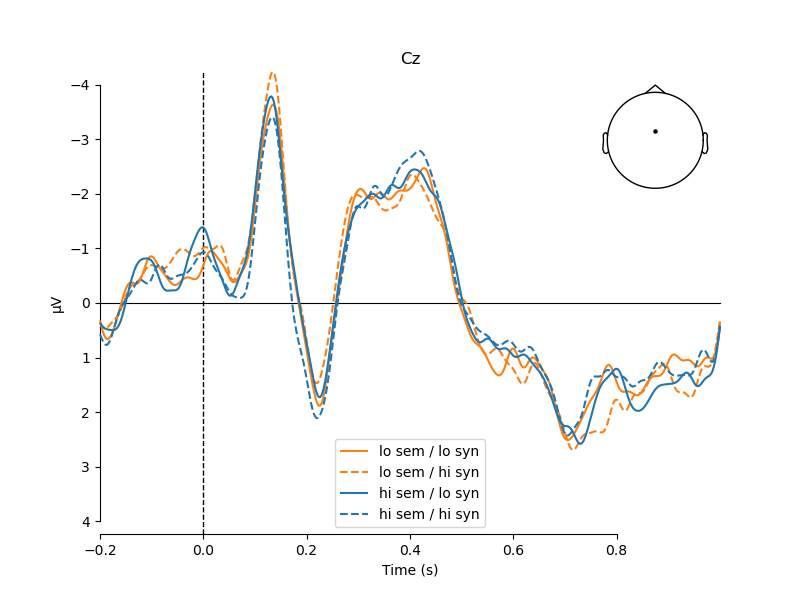
\includegraphics[width=0.95\textwidth]{images/N_103_Cz_crit.png}
\end{figure}

\begin{table}[H]
    \caption{Results from the Bayesian linear mixed model analyzing the averaged brain response from 12 centro-parietal electrodes in the time window 300 to 500 ms post critical verb onset. Baseline represents the averaged activity from the 200 ms pre-verb onset and was included in the model as a covariate instead of traditional baseline correction \citep[see][]{alday2019}.}
    \label{tab:eeg_mod}
    \centering
    \begin{tabular}{lrrr}
    \toprule
    & Estimate & Est.Error & 95\% CrI  \\
    \midrule
Intercept &  -0.70 & 0.19 &  [-1.06, -0.34] \\
baseline  &  -0.22 & 0.01 &  [-0.24, -0.20] \\
syntactic &  -0.15 & 0.08 &  [-0.32, -0.02] \\
semantic  &  -0.31 & 0.09 &  [-0.49, -0.13] \\
interaction& -0.13 & 0.10 &  [-0.37, -0.01] \\
    \bottomrule
    \end{tabular}
\end{table}

\begin{figure}[H]
    \caption{Posteriors of the syntactic and semantic interference effects and their interaction for the event-related potentials elicited by the critical verb in the spatio-temporal N400 window. Blue vertical lines represent the median and shaded areas are 80\,\% intervals.}
    \label{fig:eeg_posteriors}
    \centering
    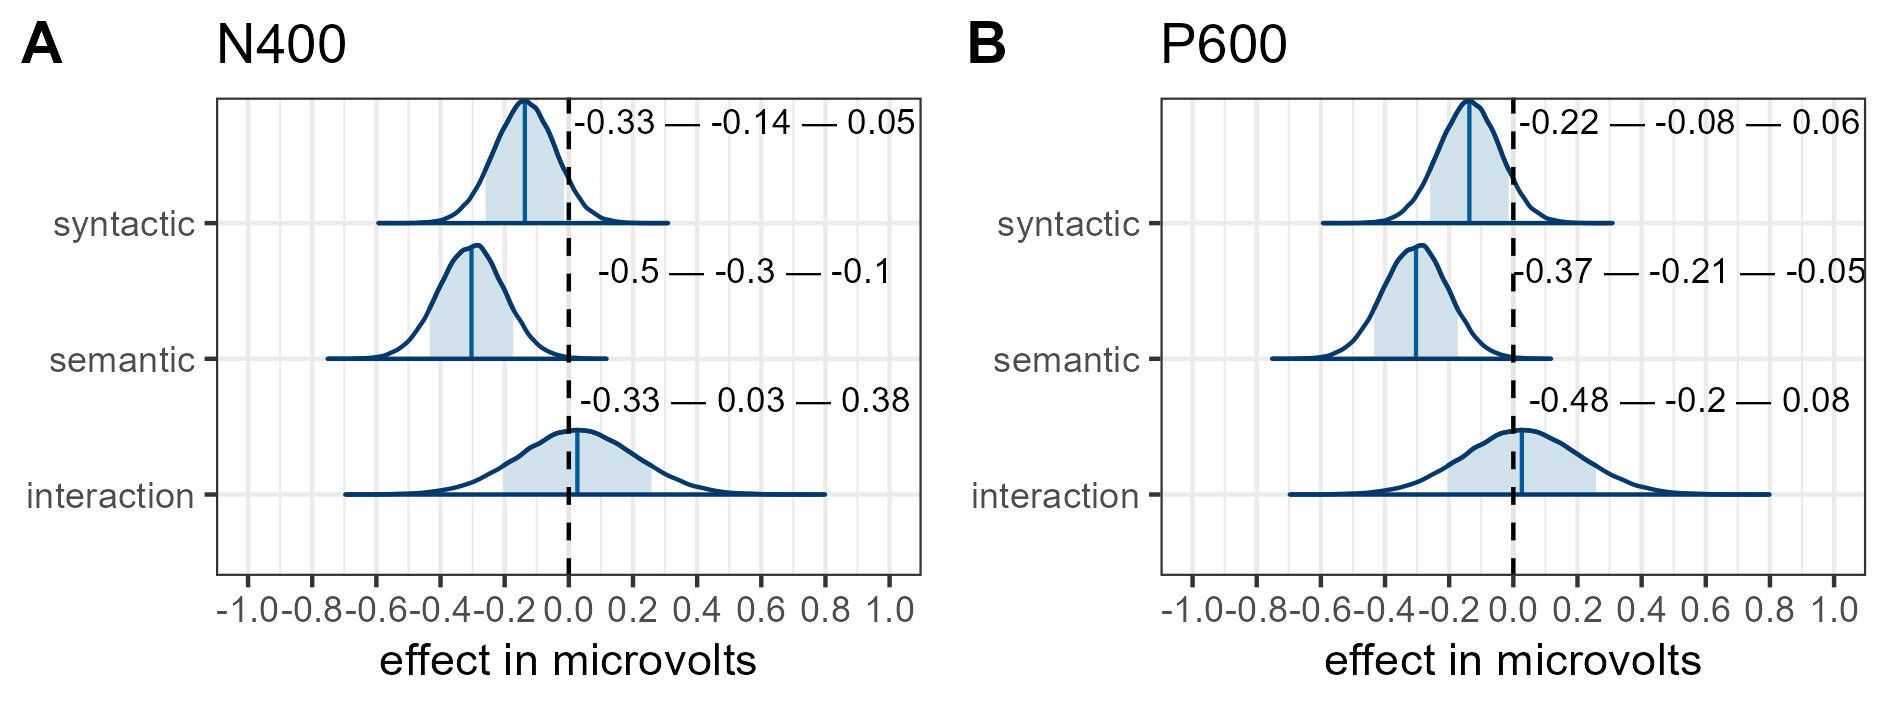
\includegraphics[width=0.6\textwidth]{images/posteriors_eeg.jpg}
\end{figure}


The semantic interference effect is further illustrated in Figure \ref{fig:erp_sem_syn} (a) and (b). Figure \ref{fig:erp_sem_syn} (a) shows that around 400 ms, the critical verb elicited a more negative ERP under high than under low semantic interference. Figure \ref{fig:erp_sem_syn} (b) shows that the topography of the effect is rather broad but with a concentration of more negative values at centro-parietal electrodes. The timing and topography of this effect suggested that it was an N400 effect, thus the N400 was modulated by semantic interference. In contrast, \ref{fig:erp_sem_syn} (c) and (d) show that syntactic interference did not considerably affect the brain response to the critical verb in the N400 spatio-temporal window. Visual inspection of the ERPs in \ref{fig:erp_sem_syn} (c) does also not suggest that there was a syntactic interference effect in any other time window.


\begin{figure}[H]
    \caption{Brain responses elicited by the critical verb. (a) ERPs for semantic interference (word onset at 0\,ms) at electrode Cz. (b) Topographic map of the semantic interference effect (high semantic interference - low semantic interference) in the N400 time window. (c) ERPs for syntactic interference  (word onset at 0\,ms) at electrode Cz. (d) Topographic map of the syntactic interference effect (high syntactic interference - low syntactic interference) in the N400 time window.}
    \label{fig:erp_sem_syn}
    \centering
         \begin{subfigure}[t]{0.74\textwidth}
         \centering
        \caption{}
         \label{fig:erp_sem_ERP}
         \includegraphics[width=\textwidth]{images/ERP_animacy_Cz.png}
     \end{subfigure}
     \hfill
     \begin{subfigure}[t]{0.25\textwidth}
         \centering
        \caption{}
         \label{fig:erp_sem_topo}
         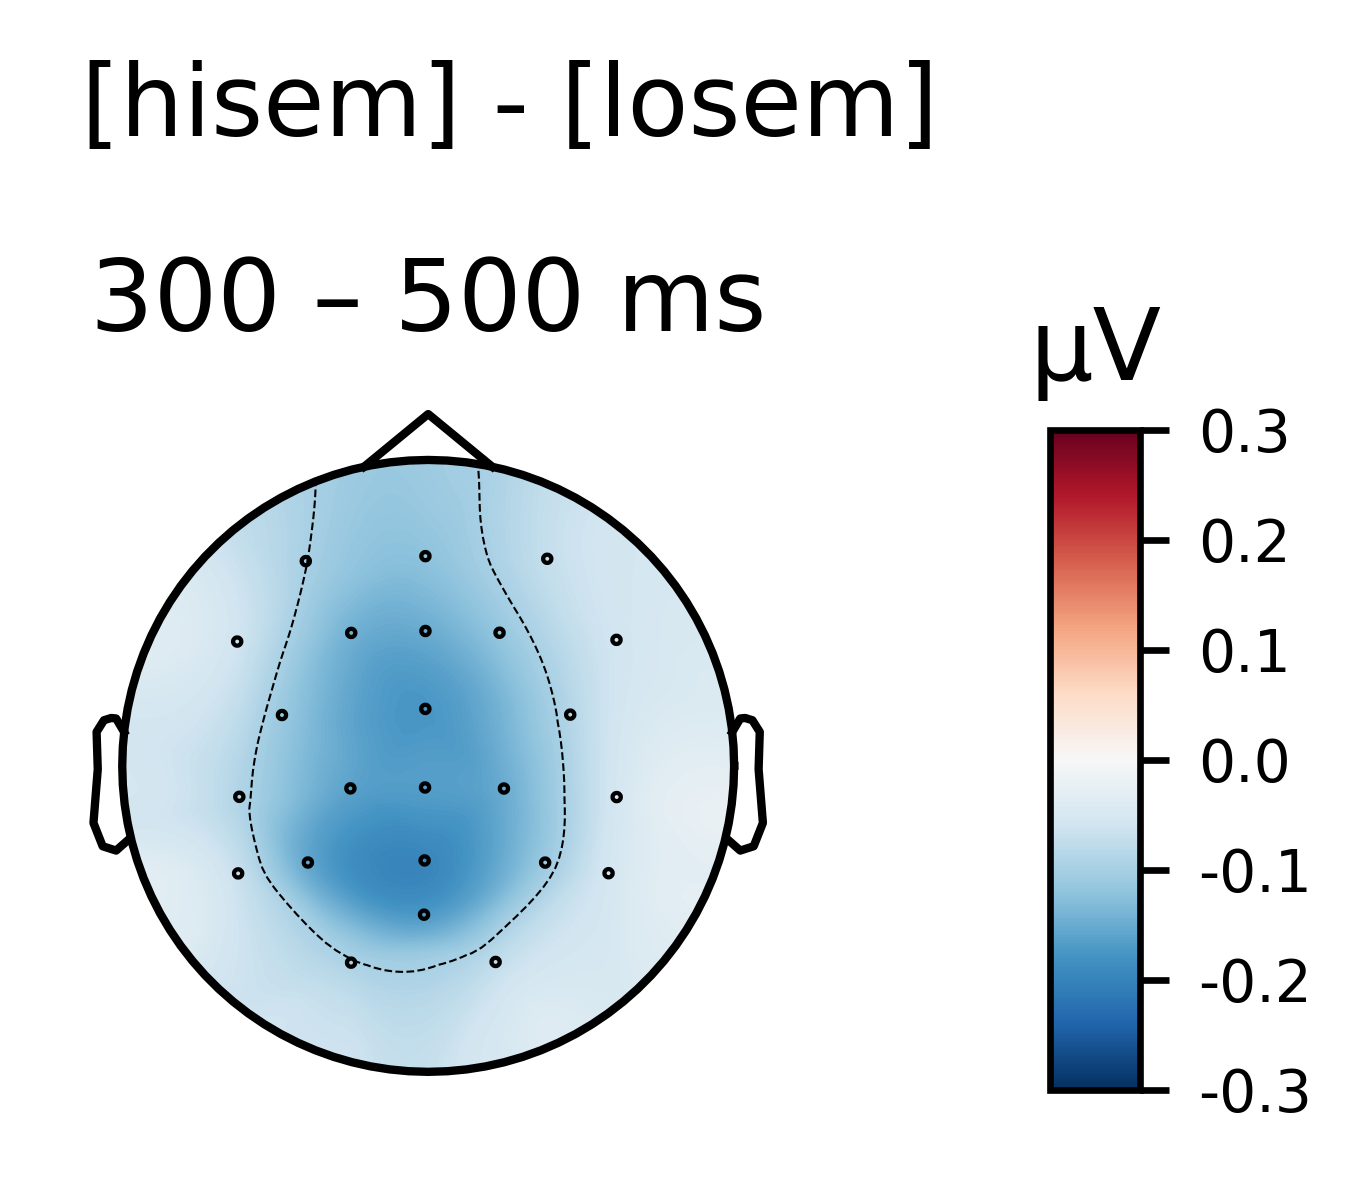
\includegraphics[width=\textwidth]{images/topo_animate-inanimate_300_500.png}
     \end{subfigure}

    \begin{subfigure}[t]{0.74\textwidth}
         \centering
        \caption{}
         \label{fig:erp_syn_ERP}
         \includegraphics[width=\textwidth]{images/ERP_subj_Cz.png}
     \end{subfigure}
     \hfill
     \begin{subfigure}[t]{0.25\textwidth}
         \centering
        \caption{}
         \label{fig:erp_syn_topo}
         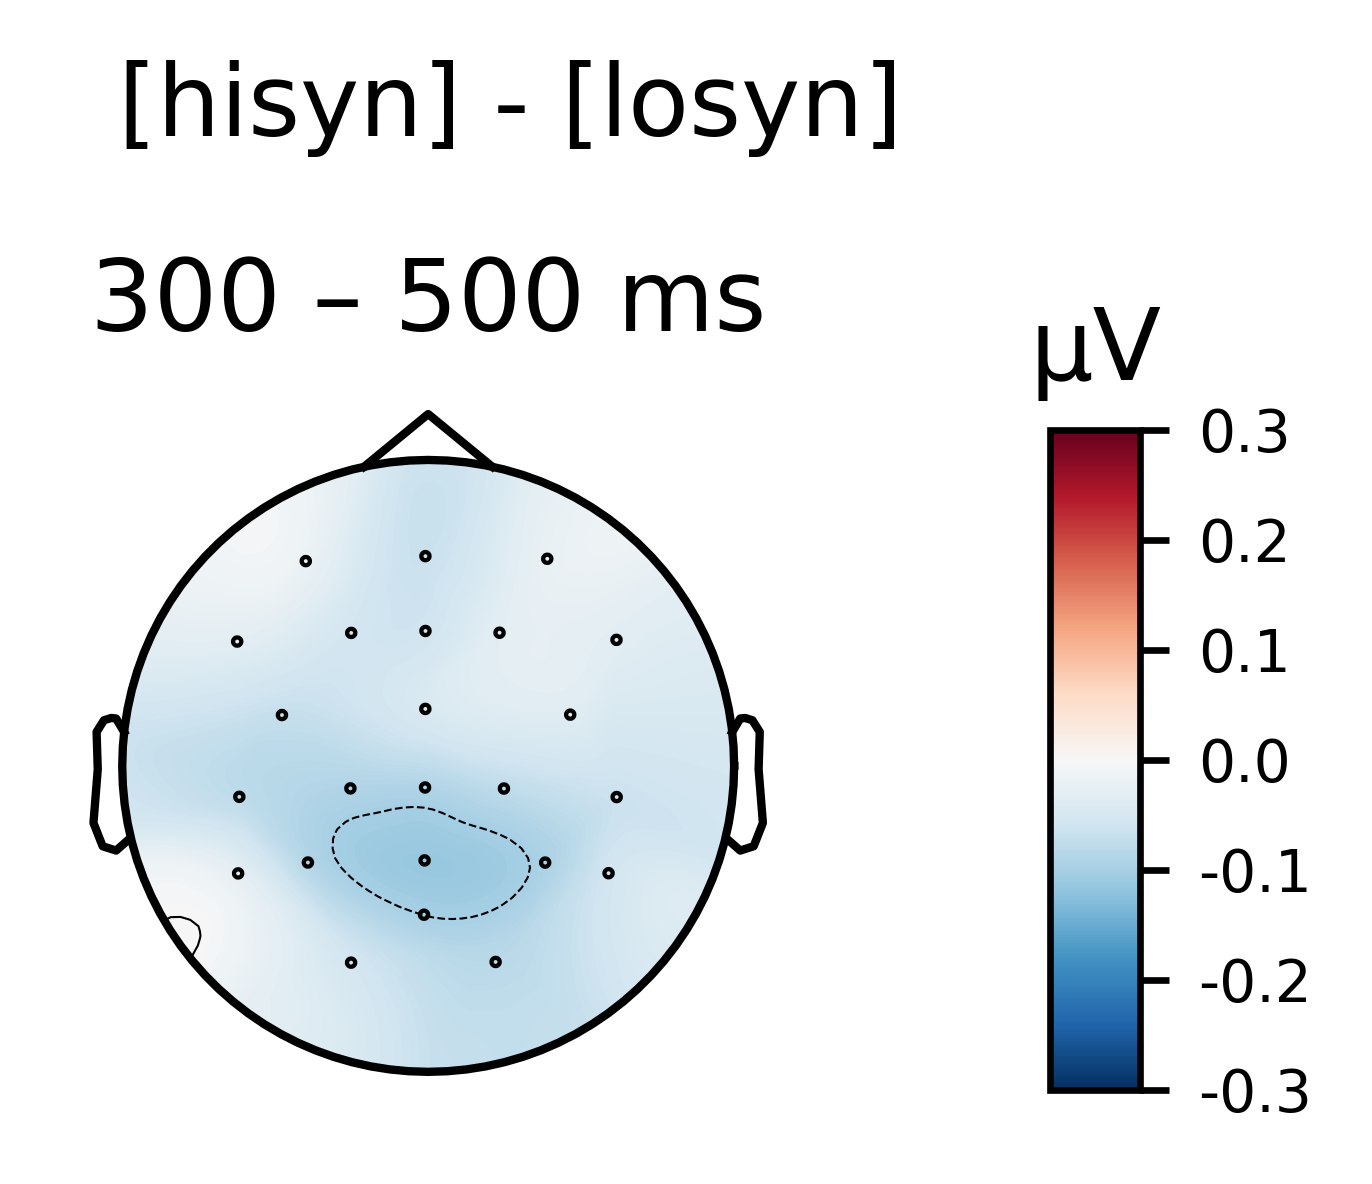
\includegraphics[width=\textwidth]{images/topo_subj-nsubj_300_500.png}
     \end{subfigure}
\end{figure} 


\paragraph{Hypothesis testing using Bayes factors}

Bayes factors are shown in Figure \ref{fig:eeg_bfs}. The Bayes factors provided very strong to strong evidence for the semantic interference effect for all priors 
(Normal$_{-}$(0, 0.1): BF$_{10}$ = 27,
Normal$_{-}$(0, 0.5): BF$_{10}$ = 88,
Normal$_{-}$(0, 1): BF$_{10}$ = 52,
Normal$_{-}$(0, 5): BF$_{10}$ = 11). 

By contrast, the syntactic interference effect had only anecdotal evidence  under the two narrow priors (Normal$_{-}$(0, 0.1): BF$_{10}$ = 2.5,
Normal$_{-}$(0, 0.5): BF$_{10}$ = 1.2). There was evidence \textit{against} syntactic interference under wider priors 
(Normal$_{-}$(0, 1): BF$_{10}$ = 0.66,
Normal$_{-}$(0, 5): BF$_{10}$ = 0.14).  What this means is that, in our data, only if we assume a priori that the effect size is relatively small, there is very weak evidence in favor of syntactic interference.

Across all priors, the Bayes factors provided evidence \textit{against} the interaction of semantic and syntactic interference (BF$_{10}$ < 0.85).


\begin{figure}
    \caption{Bayes factors for the effects of semantic interference, syntactic interference and their interaction in the time window 300 to 500 ms post critical verb onset at centro-parietal electrode sites.}
    \label{fig:eeg_bfs}
    \centering
    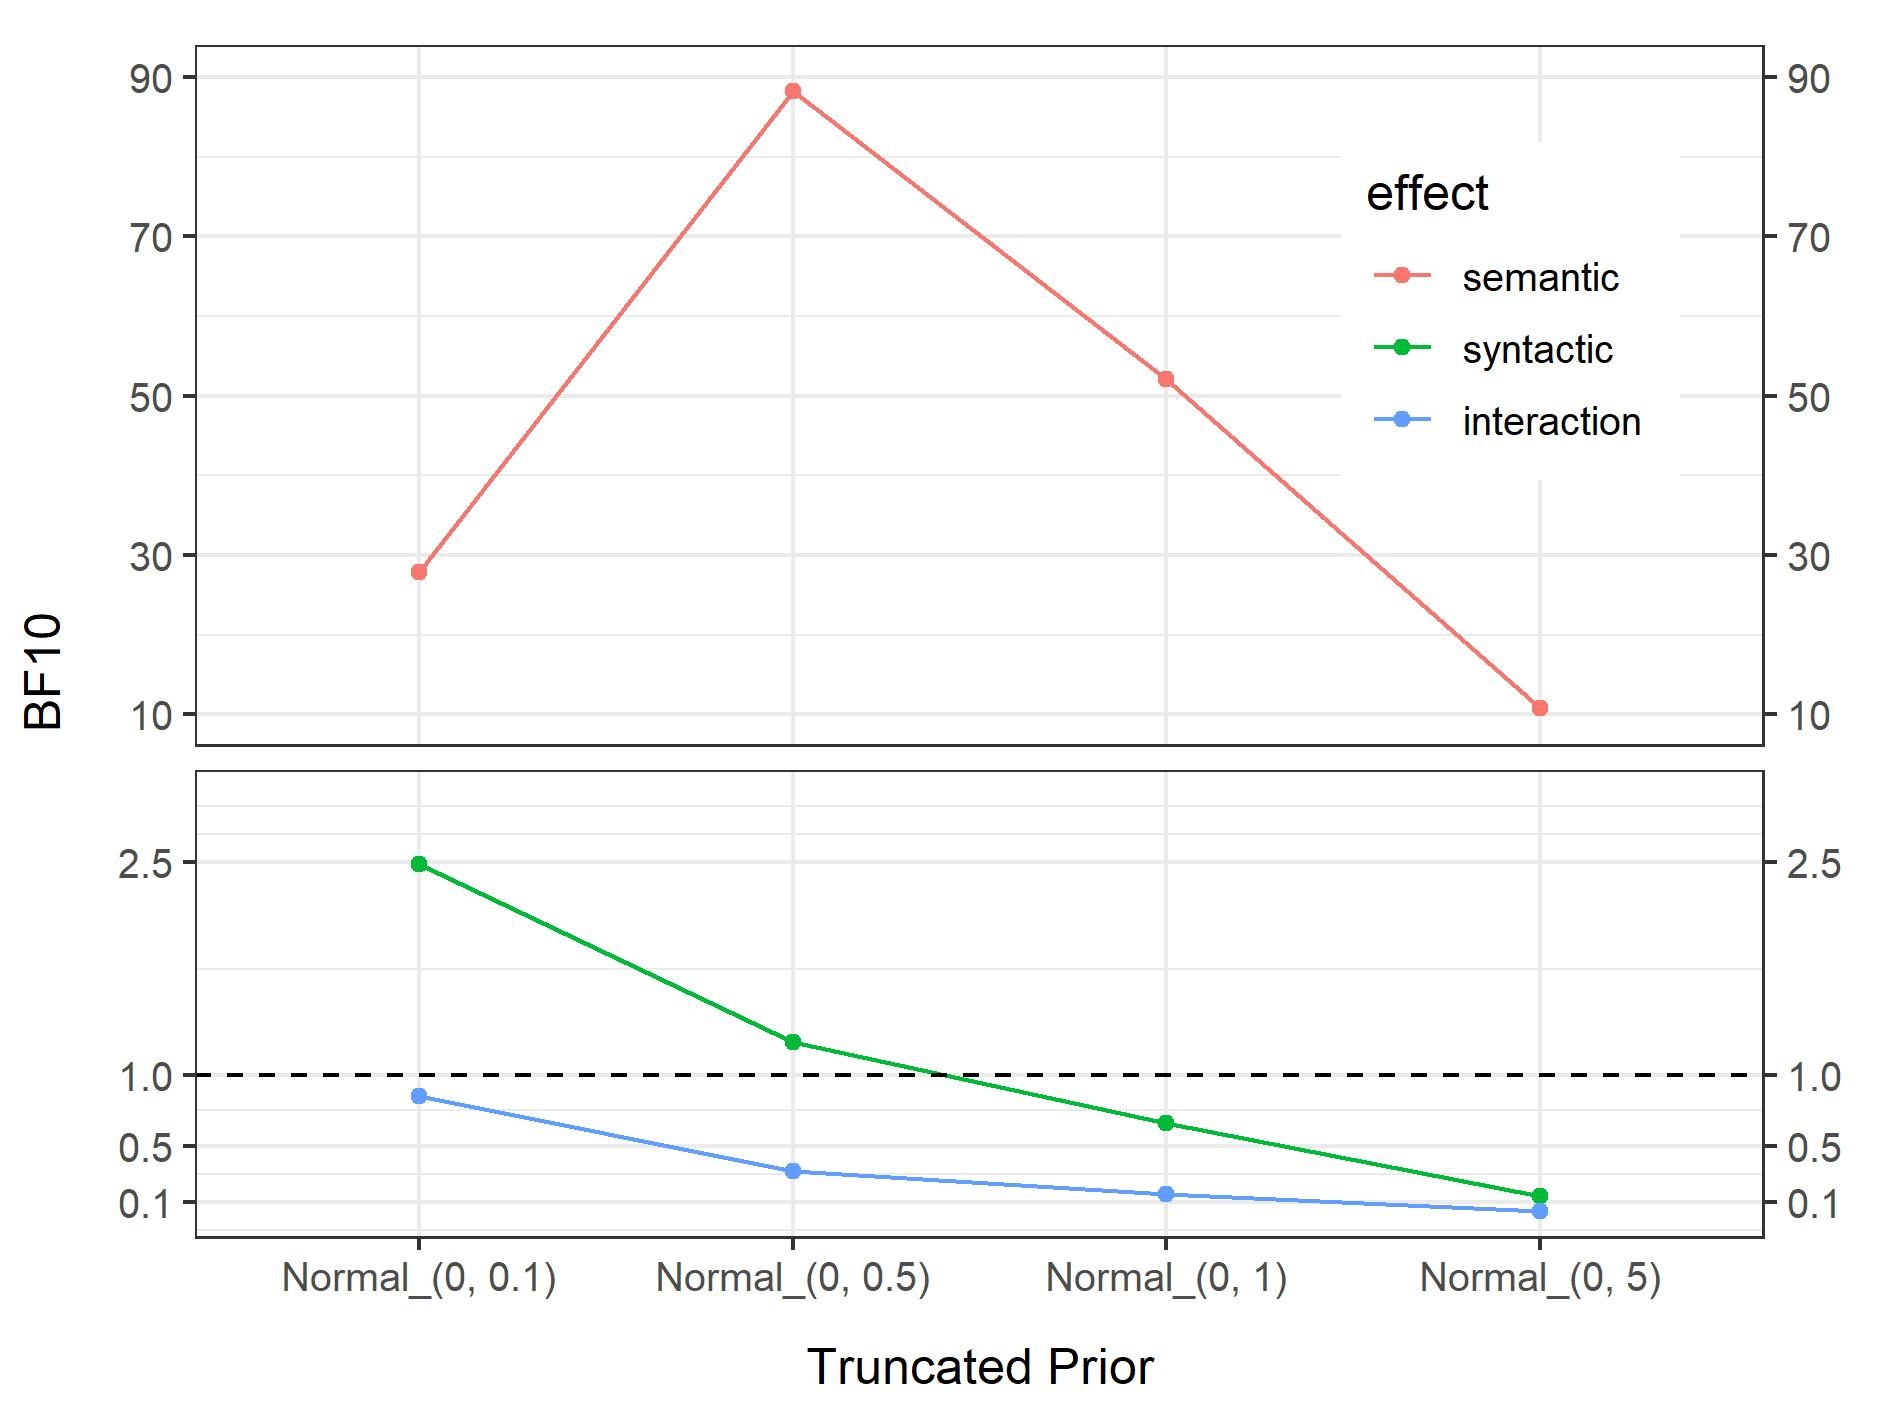
\includegraphics[width=0.9\textwidth]{images/BF_plot_N103_cp_300_500.jpg}
\end{figure}

\subsection{Discussion}
We presented a relatively large-scale ERP experiment investigating syntactic and semantic interference during subject-verb dependency completion. To our knowledge, this is the first ERP experiment on this classic interference design, which has only been investigated using reading studies so far \parencite{mertzen,vandyke07}. 

Comprehension accuracy was reduced for high vs.\ low semantic interference conditions. 
Syntactic interference itself did not affect accuracy. There was a numerical suggestion of an interaction: indicated that the difference in accuracy between low and high semantic interference conditions was larger when syntactic interference was high vs.\ when it was low (17 vs.\ 8). 

The Bayes factors analyses found strong evidence for semantic interference in the N400 amplitude. Syntactic interference had much weaker evidence in the N400 amplitude; only anecdotal evidence was found under narrow priors, and there was clear evidence against syntactic interference under wider priors. The evidence against an interaction under all priors was unequivocal. . 

Our finding that retrieval interference modulates the N400 amplitude supports the N400 as a marker of memory retrieval \citep{kutas&federmeier_2000, kutas_federmeier2011, brouwer2017_n4_p6, lau2008_n400}.

Consistent with the self-paced reading study, there is clear evidence for semantic interference, and evidence against syntactic interference.  How do these observed patterns compare to the theoretical predictions of cue-based retrieval theory? We turn to this point next by discussing the quantiative predictions of the \textcite{Lewis2005} model.

%The to date rather small body of ERP studies on interference effects during sentence comprehension gives an indeterminate picture of the nature of interference effects in ERP measures. The present study adds a large data point to the body of literature which reported negativities or more specifically N400 effects for high vs.\ low interference conditions \citep{vasishth_drenhaus_2011, martinetal2014, schoknecht2022, lee_garnsey}. Therefore, it contributes to the debate of how interference effects manifest themselves electrophysiologically (interference effects have also been reported in differences in the P600, \textcite{Tanner_etal_2017, martinetal2014}). 

\section{Quantitative predictions of the Lewis and Vasishth (2005) model for the present design}

 \textcite{mertzen} presented simulations that show approximately equally sized interference effects 
for both the syntactic and semantic manipulations. Their model assumed that three cues were used at the verb:  \{$\pm$ subject, $\pm$ same clause, $\pm$ animacy\}. The upper part of Figure \ref{fig:model_predictions} reproduces the \textcite{mertzen}   simulations. These are prior predictive distributions of the effects of interest, by sampling from a prior distribution ($Beta(a=4,b=6)$) for the free scaling parameter F and then generating data from the model while holding all other parameters in the model at fixed values. The F parameter scales the activation to a retrieval time. The prior $Beta(a=4,b=6)$ was chosen in earlier work \parencite{jaeger_etal_2020}. 

Although the semantic interference effect estimates from the SPR study fall within the predicted range from the model, the syntactic interference effect is quite divergent: as discussed earlier, the SPR data show evidence against syntactic interference, but the model predicts a syntactic interference effect of approximately the same magnitude as semantic interference. Given that the EEG data also speak against syntactic interference, it is plausible that, at least in this experimental design and language, syntactic interference plays no role. 

The absence of (and evidence against) syntactic interference is surprising because the psycholinguistic literature has clearly established that syntactic constraints play a role in sentence processing. For example, \textcite{dillon2013} and \textcite{Sturt2003} argued that principle A of the binding theory controls the retrieval process in the antecedent-reflexive dependency, effectively eliminating or attenuating interference from other overlapping features (such as number marking) of intervening nouns that cannot be an antecedent for the reflexive. For further evidence for this idea from individual differences, see \textcite{yadav2021individual}. Even more relevant to the present study is the fact that \textcite{mertzen} did find syntactic interference effects. 

Could the absence of syntactic interference be reconciled with a cue-based retrieval account? We speculated that one possibility might be that the parser tracks hierarchical structure and that this hierarchical information is used when searching for a noun in memory. Specifically, the relevant syntactic cues that might be used at the verb is not  \{$\pm$ subject, $\pm$ same clause\} but rather a composite cue  \{$\pm$ subject-in-same-clause\} . In other words, in the spirit of the  \textcite{dillon2013} and \textcite{Sturt2003} proposal, that the parser intelligently targets only the syntactically relevant noun during antecedent retrieval, we evaluated the predictions of the model assuming that the cues are   \{$\pm$ subject-in-same-clause, $\pm$ animate\}. The results of the prior predictive simulations are shown in 
the lower part of Figure \ref{fig:model_predictions}. This model now shows the observed pattern: a semantic interference effect but no syntactic interference. One limitation here is that the prior predictive distribution of our post-hoc  model still overestimates the semantic interference effect (95\,\% CrI [10, 67]\,ms; the largest effect observed the SPR studywas [4, 12] ms at the critical region). This overestimation has to do with the fact that the prior on the F parameter is relatively spread out; it would be  possible to fit the parameter to the SPR data.

The \citet{Lewis2005} model is generally used to predict reading times. The scaling factor \textit{F}  links the activation of items in memory to retrieval times \citep{Lewis2005}. But this scaling factor could be adjusted to link activation to brain responses to use the model to generate predictions on the microvolt scale for ERP data. The general effect pattern (no syntactic interference effect, but a semantic interference effect) would not be affected by an adjustment of the scaling factor. Therefore, the \{$\pm$ subject-in-same-clause \} cue instead of the \{± grammatical subject\} cue explanation can account for the estimates of the present ERP study as well.

Thus, one theoretical assumption that would be consistent with the observed SPR and EEG data is that the parser uses the animacy cue exactly as proposed in previous work on cue-based retrieval; however, the parser uses the syntactic cue while keeping track of the syntactic location of the subject.  This is of course a speculative claim that would need to be further investigated empirically. 


%There is another point to make regarding the small size of the effects observed in the present study: The observed semantic effect in self-paced reading times (8 ms, 95\,\% CrI [4, 12]) only slightly overlaps with the quantitative predictions from the \citet{Lewis2005} model of cue-based retrieval for the \citet{vandyke07} design (95\,\% CrI [9, 49]\,ms, implementation of the model by \textcite{engelmann_etal_2019}, adapted to the current design with the retrieval cues \{± animate\} and \{± grammatical subject\}). The \citet{Lewis2005} model does not only overestimate the effect size of semantic interference, but it also predicts equally sized semantic and syntactic interference effects (see Figure \ref{fig:model_predictions}). The syntactic effect is absent in our data.

%It would be implausible to argue that the absence of the syntactic interference effect suggests that the comprehender does not use syntactic information for subject-verb dependency resolution at all. We rather suggest that the \{± grammatical subject\} cue was not the right syntactic cue to investigate. In line with \citet{mertzen}, we suggest that a syntactic or structural cue along the lines of \{± same clause\} might be used during comprehension. Figure \ref{fig:model_predictions} presents the predictions of the \citet{Lewis2005} model for the \citet{vandyke07} design where additionally to the \{± animate\} cue either the canonical cue \{± grammatical subject\} or the alternative cue \{± same clause\} was implemented. The \{± same clause\} cue model does predict the syntactic interference effect to be centered around zero (95\,\% CrI [-4, 3]\,ms). This prediction is consistent with the results of the present study. However, the \{± same clause\} model still overestimates the semantic interference effect (95\,\% CrI [10, 67]\,ms).

\begin{figure}[H]
    \centering
    \caption{Prior predicted reading times for syntactic and semantic interference and their interaction from the Lewis \& Vasishth (2005) model as implemented in R by Engelmann et al.\ (2019). The upper panel shows the predictions using the three retrieval cues used in Mertzen et al.\ 2022, and the lower panel shows the predictions using the two cues \{$\pm$ subject-in-same-clause, $\pm$ animate\}. 
    The implemented model is available with the code and data provided with this paper.}
    \label{fig:model_predictions}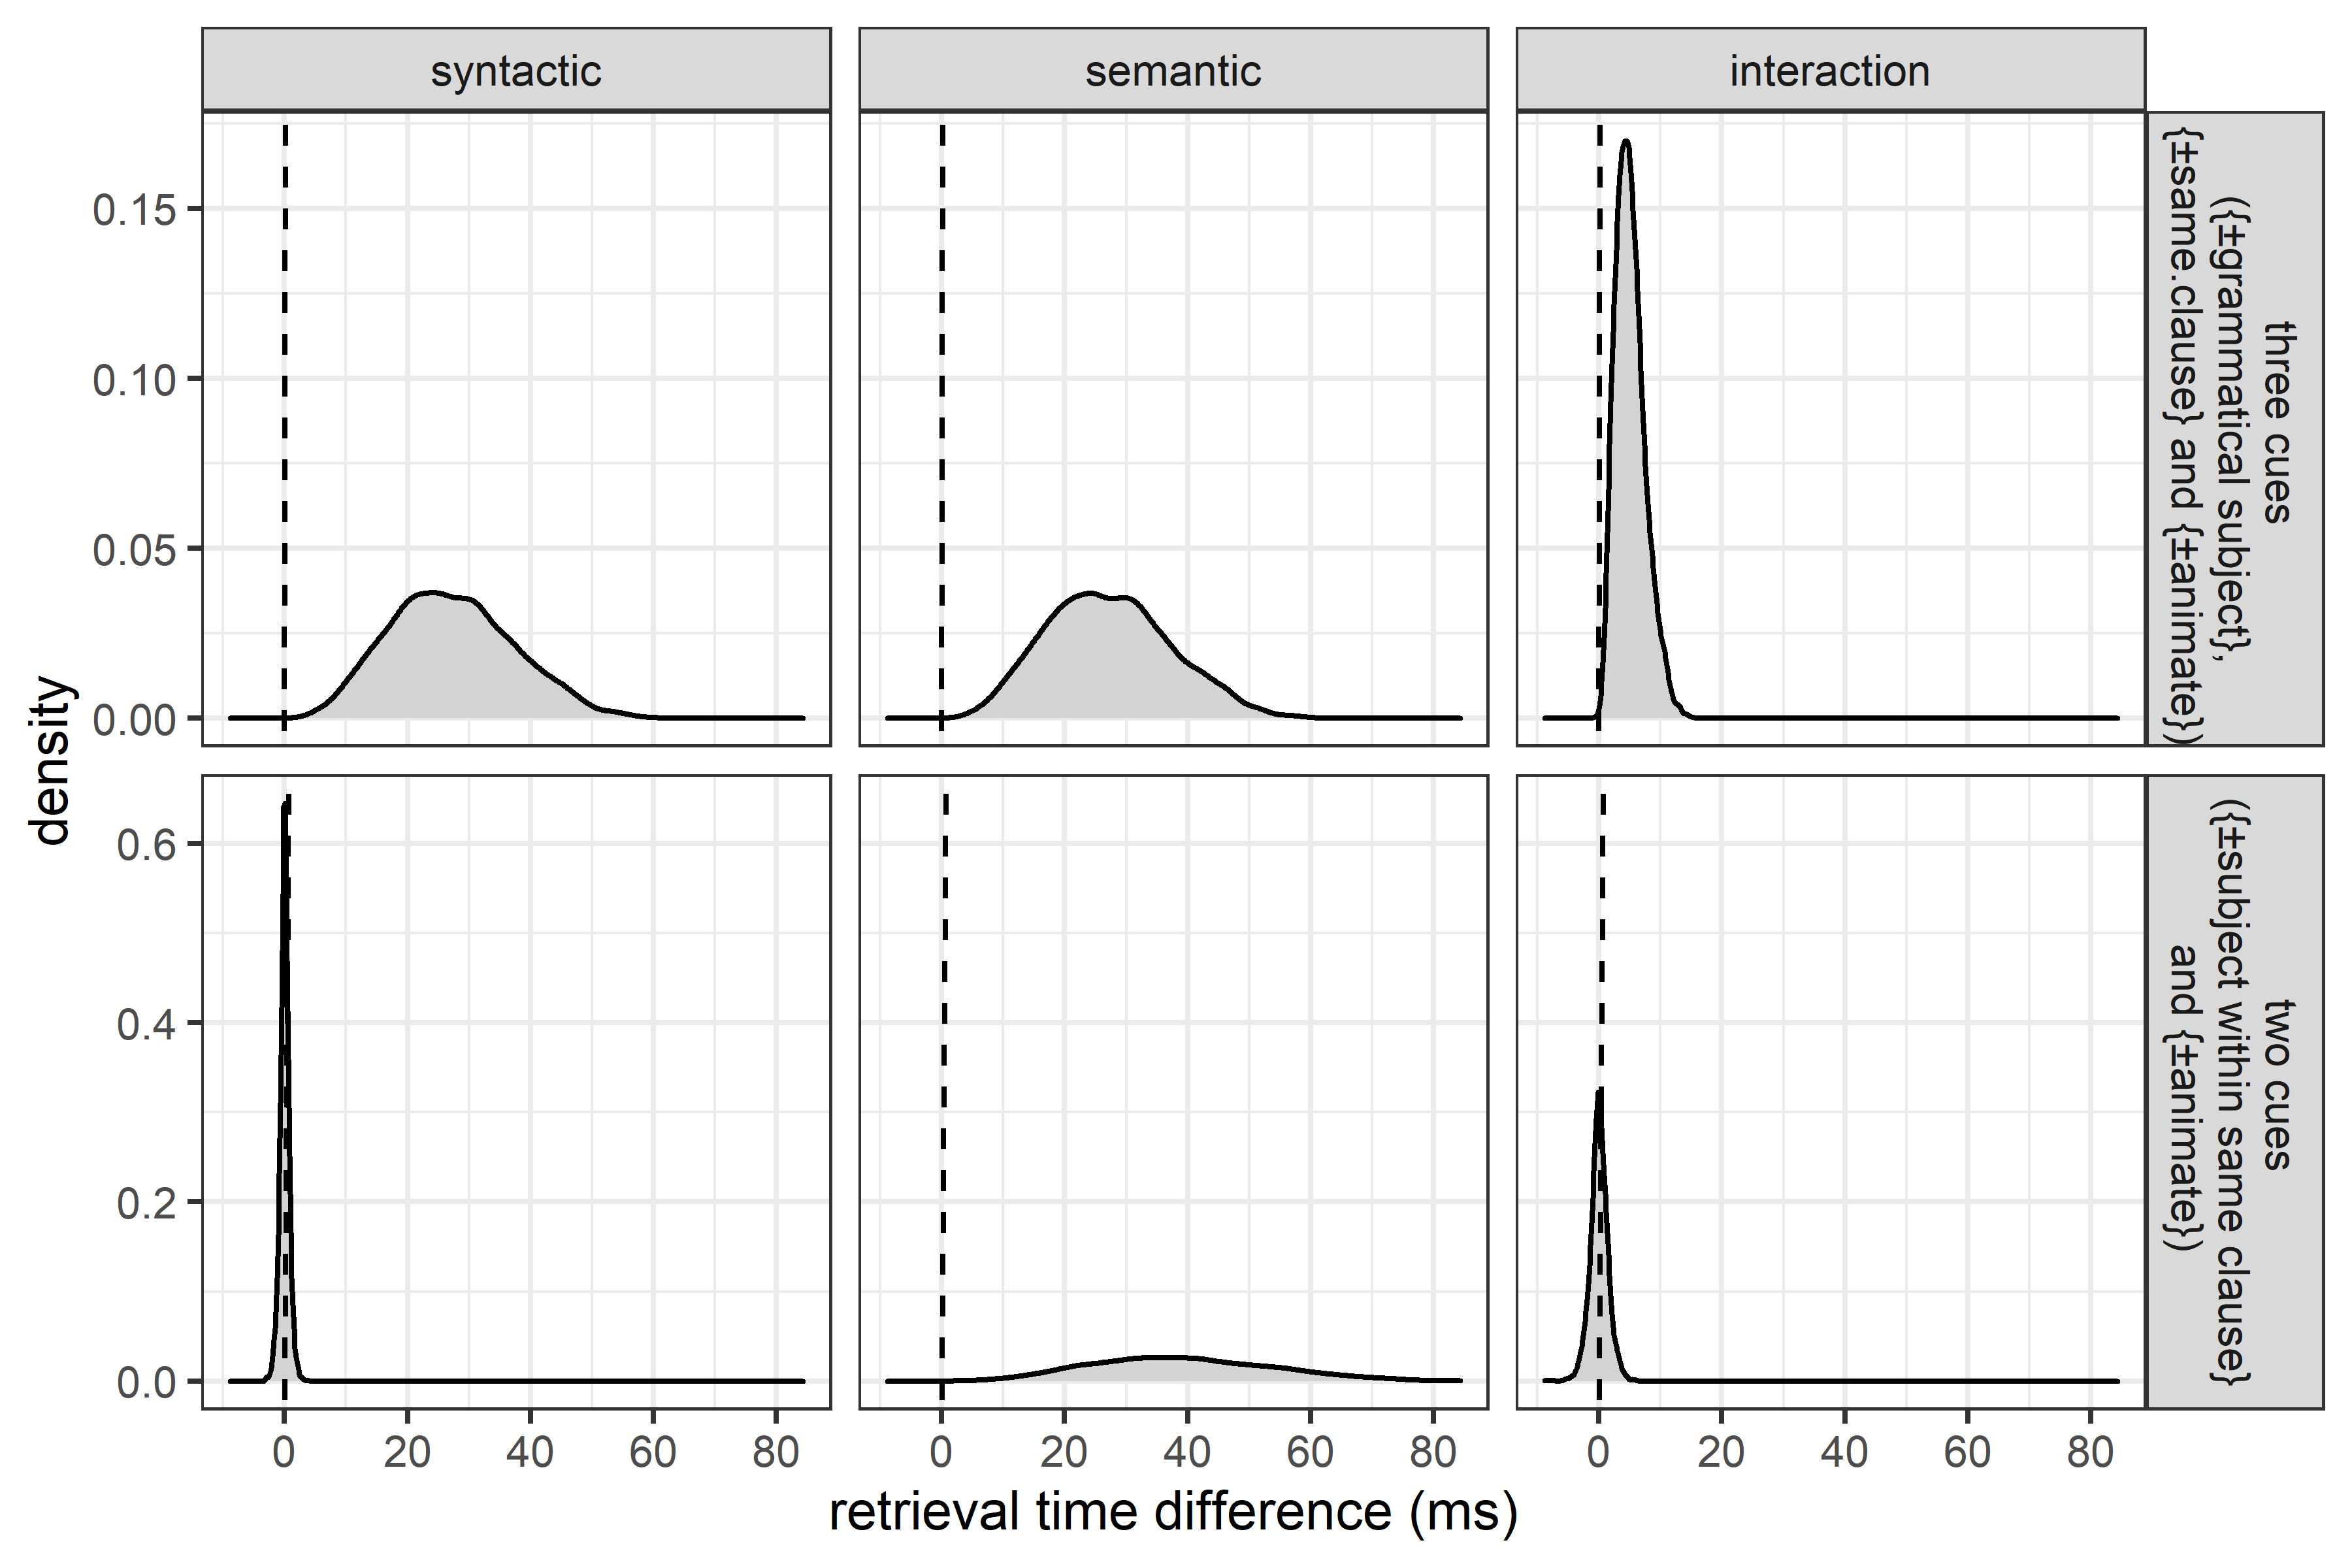
\includegraphics[width=\textwidth]{images/PriorPredicted_interACTversions_2vs3.png}
\end{figure}



\section{General discussion}

Taken together, the SPR and ERP experiments consistently showed effects of semantic interference and no effects of syntactic interference. This pattern was not only found in the dependent measures of the experiments that were of primary interest, but also in the comprehension accuracy. 
The modeling reported here suggests that one way to explain the observed pattern in the context of cue-based retrieval is by assuming that the parser intelligently searches for a subject that is within the same clause, and uses the animacy cue without reference to the clause that a noun appears in. A broader implication is that the human sentence comprehension system may be using the hierarchical syntactic structure to selectively target nouns for retrieval; this is an idea that has independent support in the literature \cite[e.g.,][]{Sturt2003,dillon2013}.

%Given the replicability / reproducibility crises in psycholinguistics \citep[see e.g., ][]{vasishth2018_signficancefilter,jaeger_etal_2020,nicenboim,}, and other (related) sciences \citep[see e.g., ][]{openscience2015_reproducibility,nicenboim_etal_2020,nieuwland_etal_2018}, the cross-methodological consistency is aston. It might be due to the very high sample sizes of the present experiments which granted the present study higher power than most comparable psycholinguistic studies. The higher power led to more precise estimates of the investigated effects with less uncertainty than in previous studies. 
%This also partially explains the comparatively smaller effect sizes in the present experiments than have been previously reported.

In the remainder of this section, we discuss two important issues that relate to previous experiments that investigated syntactic and semantic interference. The first is the role of encoding vs.\ retrieval interference, and the second is broader implications of our findings in the context of previous related work.

\subsection{Encoding and retrieval interference}
In the SPR data, we found that the semantic interference effect originated at the distractor and persisted throughout the following regions. Due to this time course, encoding interference \parencite{Yadavetal2022,hammerly2019grammaticality} is the best explanation for the interference effect in the reading times at the critical region. This raises the question whether the ERP effect was also caused by encoding interference, i.e., whether the ERP effect originated prior to the critical region. To answer this question, it is necessary to look at the ERPs elicited by words earlier in the sentence, This is an unusual step in ERP research but makes sense as an exploratory step in the present context. Figure \ref{fig:erp_precrit} shows the ERPs for all conditions at the critical word and the two pre-critical adverbs which were identical across conditions. It is apparent from the ERPs of the pre-pre-critical and pre-critical word that the semantic interference effect found at the critical verb was not present at the words preceding it. 

\begin{figure}[H]
    \caption{ERPs elicited by the pre-pre-critical adverb (word onset at -1800 ms), pre-critical adverb (word onset at -900 ms) and critical verb (word onset at 0\,ms) at electrode Cz.}
    \label{fig:erp_precrit}
    \centering
    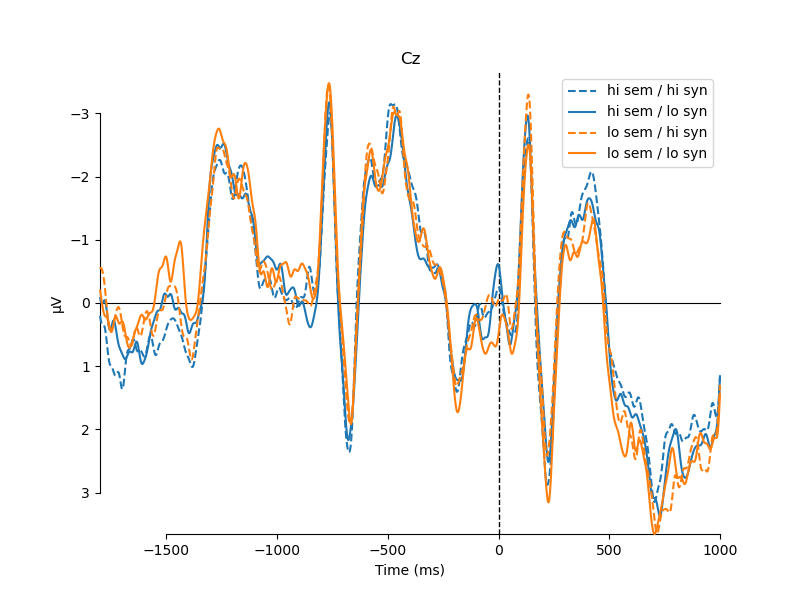
\includegraphics[width=0.95\textwidth]{images/N_103_Cz_precrit.png}
\end{figure}

Thus, the words directly preceding the critical verb do not show a pattern consistent with semantic interference. A further question that arises is: which brain response was elicited by the distractor itself (see Figure \ref{fig:erp_distractor})? An exploratory visual inspection of the ERPs elicited by the distractor shows several differences between conditions, but no semantic interference effect in the N400 spatio-temporal window. We believe that the differences in the ERPs elicited by the distractor in the different conditions are caused by two factors. First, the high and low syntactic interference conditions have different word orders, i.e., the distractors are embedded in different phrase structures (simple noun phrase vs.\ noun phrase including an adjective within a prepositional phrase; see Example \ref{ex:materials}). This is also apparent from the large difference between high and low syntactic interference conditions before distractor onset. Second, the distractors were not identical across conditions, therefore the ERPs in Figure \ref{fig:erp_distractor} are elicited by different words in the high vs.\ low semantic interference conditions. In summary, this exploratory analysis suggests that the distractors did induce different brain responses across conditions, but these could be due to factors other than encoding intererence. More importantly, these effects did not linger throughout the rest of the sentence (see Figure \ref{fig:erp_precrit}). 

\begin{figure}[H]
    \centering
        \caption{ERPs elicited by the distractor (word onset at 0 ms) at eight selected electrodes.}
    \label{fig:erp_distractor}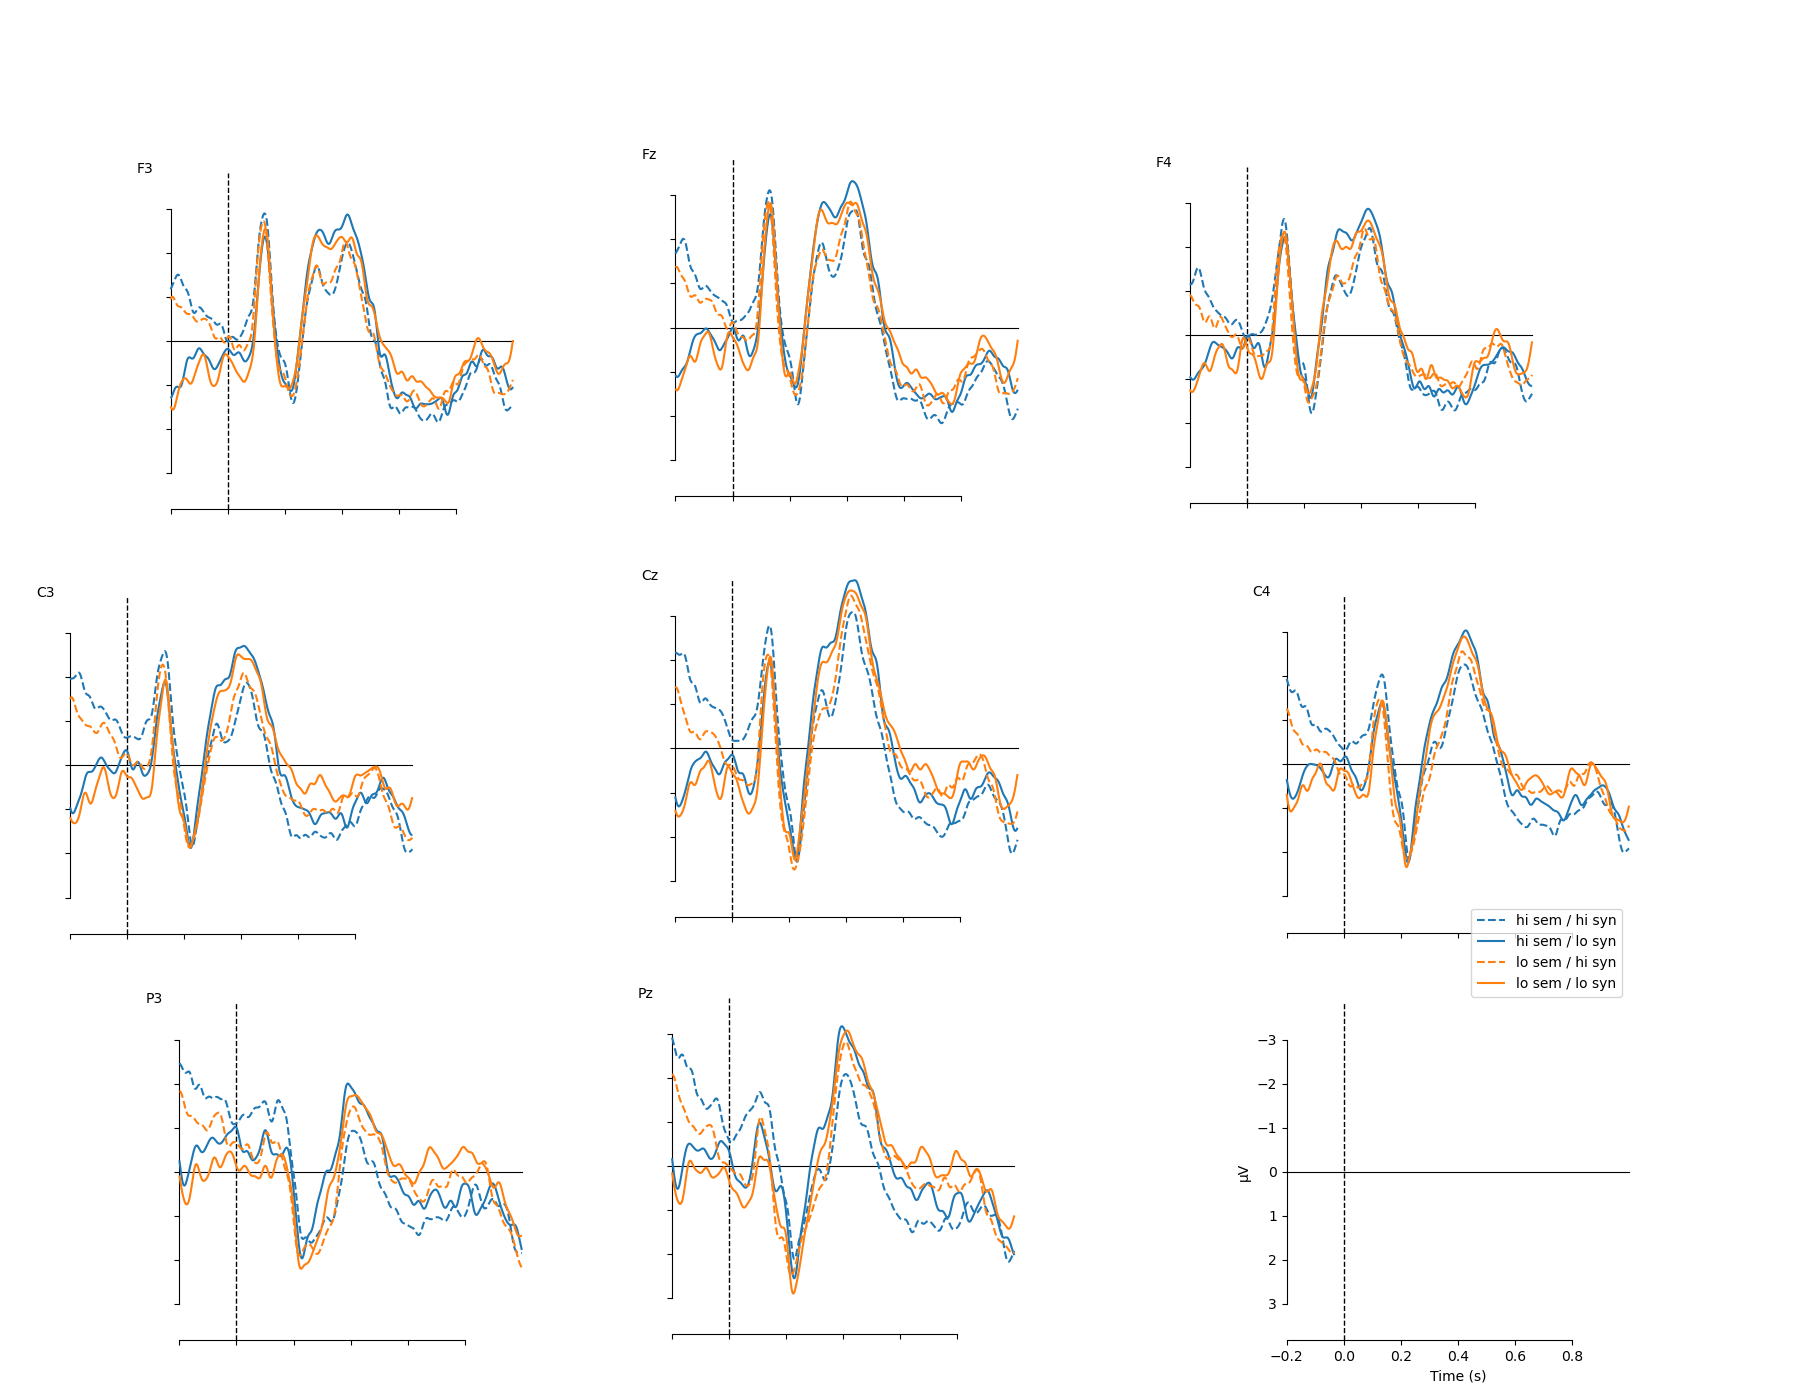
\includegraphics[width=\textwidth]{images/Distractor_N_100_some_elec.png}
\end{figure}

The comparison of the results of our SPR and ERP experiments suggests that the SPR results were strongly affected by encoding interference, while the ERPs elicited by the critical verb were not. This difference between methods might be caused by the difference in presentation rate. In the self-paced reading experiment, as implied by the name, the participants had control over the presentation rate of the stimuli. The observed slowdown starting at the distractor  might have resulted from the probably subconscious intent to slow down the sampling rate of the incoming stimuli to gain more time to process them. In contrast, in the ERP experiment, we used rapid serial visual presentation (RSVP), which presents stimuli at a fixed rate that is beyond the control of the participant. Therefore, they must adapt to the set rate and process the stimuli as fast as the rate requires. Here, it is noteworthy that the presentation duration of 500\,ms per word and 400\,ms between words which was used in the present ERP experiment is slower than usual natural reading speed. However, while in SPR the slowdown due to encoding and maintaining the distractor in memory overshadowed potential retrieval effects, the procedure of the ERP experiment might have prevented that. In the ERP results, we observed an effect at the critical verb, which could be attributed exclusively to the retrieval process hypothesized by cue-based retrieval accounts. Having said that, we cannot rule out the possibility that--due to the auto-paced nature of the ERP experiment--any encoding interference that started at or after the distractor is mixed in with the cost of retrieval interference. Indeed, recent modeling work on agreement attraction in reading \parencite{Yadavetal2022} has shown conclusively that some kind of feature distortion as well as cue-based retrieval are needed to explain the benchmark data-sets that exist so far on agreement attraction in reading. If the  \textcite{Yadavetal2022} extends to interference effects in general, 
it is reasonable to assume that the effect observed at the verb in the ERP study is driven by both encoding and retrieval interference. However, we cannot resolve the relative roles of these latent processes in the present study.

\subsection{Relation to other sentence processing accounts}

%Besides our considerations above regarding the possibility that another syntactic cue (e.g., \{± same clause\}) was used, our results highlight the importance of the semantic cue for subject-verb dependency resolution.

The evidence against a main effect of syntactic interference for subject-verb dependency resolution in our study is not consistent with the assumption in previous work, e.g., \textcite{vandyke07,mertzen}, that the parser searches for a subject simply by setting the retrieval cue \{± grammatical subject\}.
  However, the semantic interference effect we found can be easily reconciled with previous work in  sentence processing. In the modeling section above, we have already discussed how our results relate to predictions from the \citet{Lewis2005} cue-based retrieval model.  
  %Our results may also be consisted with constraint-based models \citep[e.g.,][]{macdonald1994, mcrae1998modeling, trueswell1993}. Under constraint-based accounts, it is assumed that multiple constraints simultaneously and immediately influence processing. These accounts predict our ERP results: Compared to an inanimate distractor, an animate distractor -- regardless of its syntactic status -- would impede processing at a verb which requires an animate subject. The lack of a syntactic interference effect could indicate that the status `grammatical subject' was not used as a syntactic constraint. As discussed above, a plausible syntactic constraint is that a verb and its arguments need to be within the same clause. 
 Our results could also be seen as consistent with the good-enough processing account \citep{ferreira2007goodenough}, which assumes that comprehenders do not always aim to build a fully fleshed-out analysis of a sentence, but instead might accept incomplete, underspecified, or even incorrect analyses. The high number of participants that needed to be excluded in our experiments due to accuracy below 70\,\% (117 out of 908 participants in the SPR experiment, 29 out of 146 participants in the EEG experiment), suggests that our materials led to high processing demands. It is reasonable to assume that the participants might have--at least occasionally--adopted a good-enough processing mode when faced with high task demands \parencite{swets2008underspecification,LogacevMultiple,LogacevVasishthQJEP2016} or due to working memory capacity limitations \parencite{MalsburgVasishth2013}, or both. So, given a good-enough processing mode which leaves some syntactic relations within the sentence underspecified, it makes sense for the comprehender to use a simple heuristic for subject-verb dependency resolution. Animacy is an obvious choice for such a heuristic. Animate entities are proto-typical agents \citep{dowty1991thematic} and therefore, the primary use of the \{+ animate\} cue to retrieve a subject leads to the correct analysis with high probability (not just within the experiment context, but in everyday language use). Finally, our findings are also consistent with the possibility that language processing relies predominantly on semantic associations to form (probabilistic)
representation of event structures. This view has been put forward by \textcite{rabovsky_etal_2018}, when they used the neural-network sentence gestalt model \parencite{mcclelland1989_sentence_gestalt}, to model the N400 amplitude. This model assumes that language comprehension relies on associative form-to-meaning mapping instead of syntactic rules. This assumption is consistent with our results.

Without the modeling results reported above, it would be easy to conclude that our data show that  syntactic cues play no role in sentence processing. However, this conclusion would be obviously wrong. First, as we showed above, the retrieval model suggests that--at least in our data--the subject cue is used, but differently than previously assumed: the relevant cue may be subject-in-same-clause. Second, there is plenty of independent evidence for the central role of syntactic information in comprehension; some examples are the role of case marking \parencite[e.g.,][]{ALV2019,HusainEtAl2014,bhatia2022processing,bader2000case,bader2006case,miyamoto2002case}, syntactic constraints like Principle A of the binding theory \parencite[e.g.,][]{Sturt2003,dillon2013,yadav2021individual},  and 
the importance of word order \parencite[e.g.,][]{meng2000mode}. There are of course important examples of the parser ignoring syntactic information. Three dramatic examples are the grammaticality illusion in multiple embeddings in English \parencite{gibsonthomas99}, the agreement attraction phenomenon across different languages \parencite{wagersetal,lago_etal_2021,jaeger_etal_2017}, and local coherence effects \parencite{taboretal04}.  However, there are languages (such as German and Dutch) in which the grammaticality illusion does not occur \parencite{VSLK11,FrankEtAl2015}, and a large-sample study \parencite{lcpaape2023} presents evidence against the syntactic local coherence effect that was reported by \textcite{taboretal04}. Also, there seems to be at least one language that has rich case marking (Czech) that does not show any evidence of agreement attraction \parencite{chromy2023number}. Thus, it seems that, cross-linguistically, the role of syntax in building incremental structure and in completing dependencies remains as important as ever.

\section{Conclusion}
%The present large-scale self-paced reading study examined the role of syntactic and semantic features during sentence comprehension. At a verb that initiated retrieval of its subject, high semantic interference led to longer reading times than low semantic interference, but only when syntactic interference was high as well. This result provided empirical support for the assumption that different types of cues are used simultaneously during memory retrieval in subject-verb dependency formation. Furthermore, it suggests that distractors must match all available retrieval cues to cause similarity-based retrieval interference. The results of the present study are similar to the predictions of cue-based retrieval models of sentence processing with non-linear combinatorics.

This project investigated the use of  syntactic and semantic cues during subject-verb dependency resolution with self-paced reading and event-related potentials.  Both our experiments consistently showed semantic interference, i.e., more processing difficulty during long-distance subject-verb dependency resolution in the presence of a semantically matching distractor. This manifested in longer self-paced reading times starting at the distractor and continuing into the post-critical region, and in a more negative N400 amplitude for the high vs.\ low semantic interference conditions elicited by the critical verb. These different time courses in the two experiments are likely to be due to different types of interference: Encoding interference in the SPR experiment and retrieval (and possibly also encoding) interference in the ERP experiment. These differences in the time course are likely to be due to the methods used in the two sets of experiments (self-paced vs.\ auto-paced reading). Overall, we found evidence against the use of a syntactic cue such as \{$\pm$ grammatical subject\}, as previously assumed in the literature; computational modeling shows that the most likely explanation for the observed data is that the parser uses the syntactic cue  \{± subject-in-same-clause\}  to identify the correct target for retrieval.  A broader implication is that the parser may be able to use hierarchical structure in the input to intelligently target the correct syntactic dependent from memory, leading to no interference from a distractor that is in subject position within an embedded clause.

\section{Data availability statement}

The data and analysis scripts can be accessed via https://osf.io/4fpru/?view$\_$only=.


\newpage
\printbibliography

\appendix 

\section{Previous work on syntactic and semantic interference in reading}

But are both syntactic and semantic cues used during memory retrieval? \citet{vandyke07} and \citet{mertzen} investigated the effects of syntactic and semantic interference during long-distance subject-verb dependencies (see Example \ref{ex:1_vandyke07}) in a series of self-paced reading and eye-tracking while reading experiments. Overall, the original study by \citet{vandyke07} and the replication by \citet{mertzen} showed relatively consistent results. They consistently found syntactic interference but only rarely semantic interference (only in some measures of some of the experiments and sometimes in regions outside of the critical region). These results are not in line with the predictions from the standard cue-based retrieval models \citep{Lewis2005, mcelree}: While both previous studies found effects of syntactic and semantic interference, they emerged in different regions -- sometimes even prior to the retrieval site. Figure \ref{fig:previous} gives an overview of the previous findings. See the appendix for a detailed discussion of the previous results.

One possibly problematic aspect of the studies from \citet{vandyke07} and \citet{mertzen} is that effects were found in pre-critical regions. \citet{mertzen} suggested that the pre-critical effects could be due to structural confounds, encoding interference, preview effects during natural reading in the eye-tracking experiments or anticipatory retrieval at the pre-critical word because participants could predict that the verb would follow. It is unclear from the previous studies when exactly the pre-critical effects emerged, i.e., when the conditions started to differ. But it is important to know the timecourse of the pre-critical effects to determine their cause. If the structural confounds explanation is correct, then the pre-critical effects should appear only in relation to the syntactic manipulation. For the encoding interference explanation to be correct, it would be necessary that conditions start to differ at (or shortly after) the distractor. The preview and anticipatory retrieval explanations can only apply if the pre-critical effects are found only close to the critical verb.

The previous estimates had relatively wide 95\,\% confidence/credible intervals in some of the experiments, which is probably due to the relatively small sample sizes. \citet{vandyke07} had a typical number of participants and items for psycholinguistic experiments (35 - 40 participants per experiment, 36 - 48 items per experiment). \citet{mertzen} used the same number of items as \citet{vandyke07}, but larger participant sample sizes (English: N = 61, German N = 121). Large uncertainty raises the possibility of Type M errors, leading to misleading conclusions \citep{gelman_carlin}.  

\begin{figure}[H]
    \caption{Overview of previous findings of syntactic and semantic interference and their interaction by \citet{vandyke07} (three experiments in English with 35, 36 or 40 participants) and \citet{mertzen} (one experiment in German with 121 participants, one experiment in English with 61 participants). Experiments used either Self-paced Reading (SPR) or Eye-tracking methodology (Eye-Tracking measures: FPRT = first-pass reading time, RPD = regression-path duration, TFT = total fixation time). Error bars are 95\% confidence intervals for \citet{vandyke07} and 95\% credible intervals for \citet{mertzen}. }
    \label{fig:previous}
    \centering
    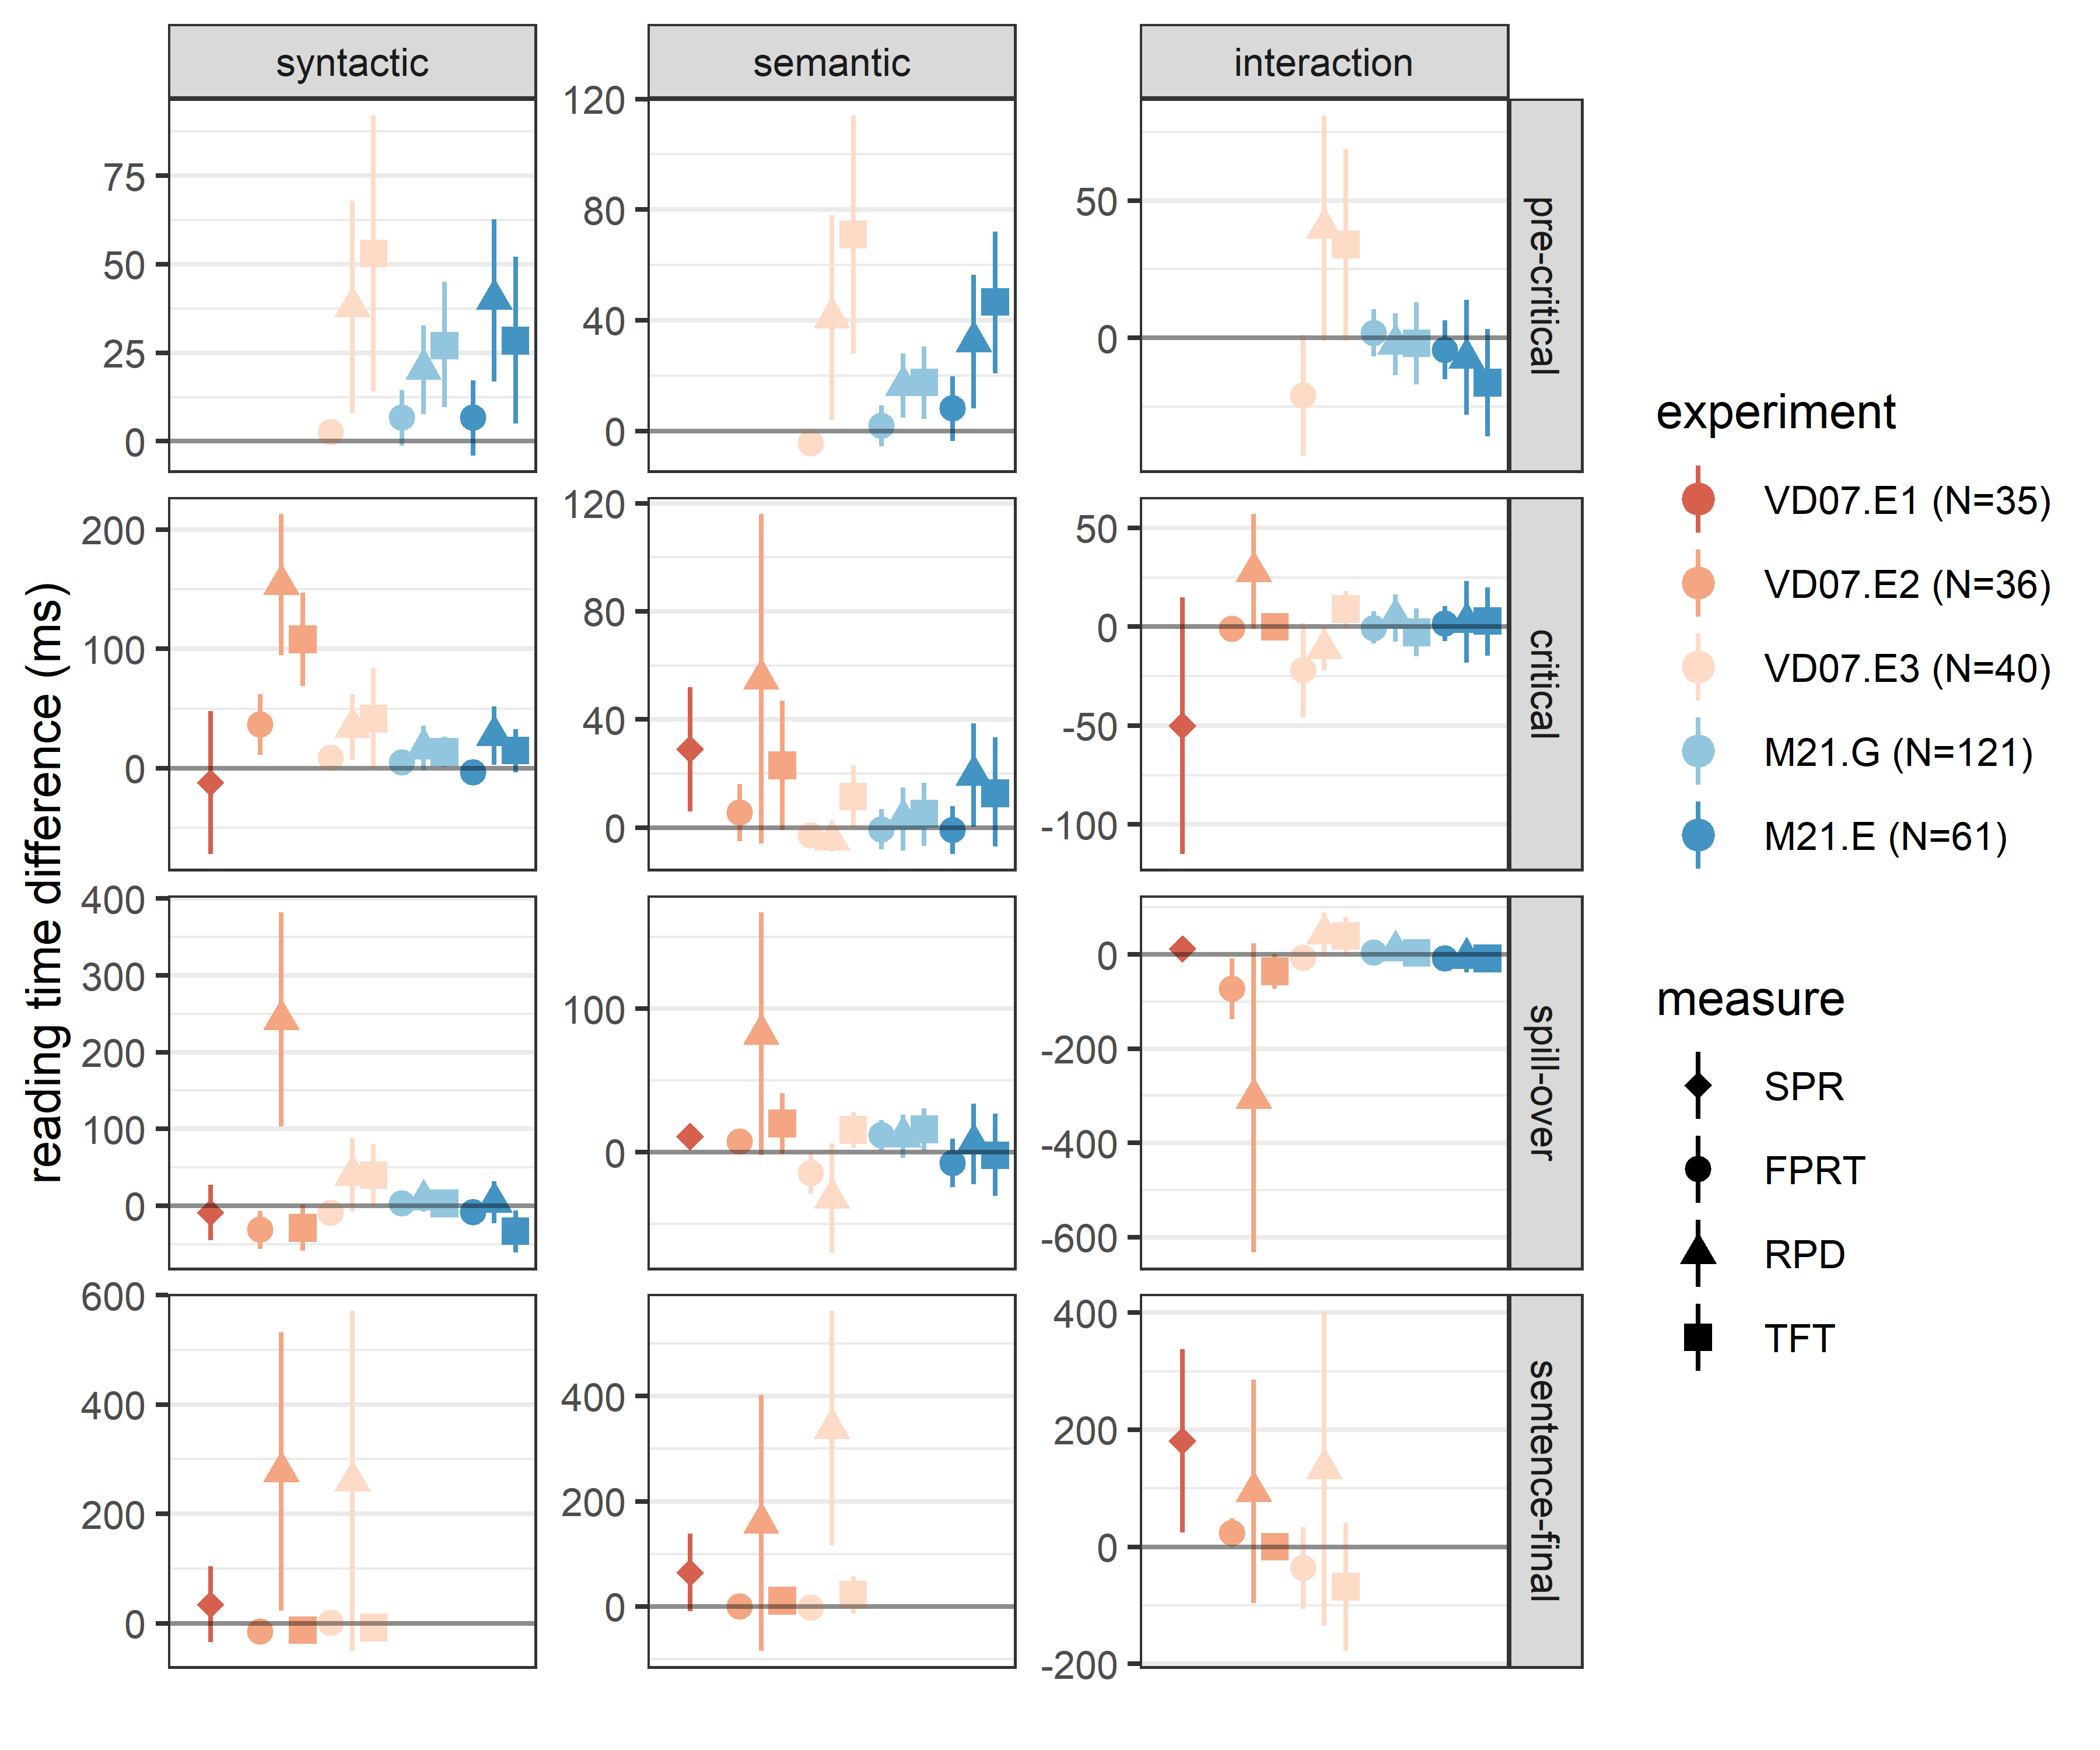
\includegraphics[width=0.95\textwidth]{images/previous_findings_allregions_long.png}
    \figurenote{The estimates for \citeauthor{vandyke07}'s (\citeyear{vandyke07}) data were derived form the published paper. For non-significant effects, where no statistics were reported, we used a t-value of 1.95 to compute the confidence intervals. \citet{mertzen} provided their estimates and credible intervals.}
\end{figure}

The results of the previous studies raise two questions: 1) Why were semantic interference effects found less consistently than syntactic interference effects? 2) Why were effects of retrieval interference observed in the pre-critical region? To answer question 1, we decided to run large-sample studies revisiting \citeauthor{vandyke07}'s (\citeyear{vandyke07}) design to gain more precise estimates of the effects of syntactic and semantic interference. To answer question 2 -- or to disentangle the possible causes of the pre-critical effects -- we decided it is best to use methods which provide responses which are unambiguously related to the processing of single words. The methods of our choice being self-paced reading (SPR) and electroencephalography (EEG) or event-related potentials (ERPs), respectively, with typical rapid serial visual presentation (RSVP) of single words. Both these methods provide responses directly linked to the processing of single words and, unlike eye-tracking while reading, do not grant any preview of upcoming stimuli. To reduce the structural confound at the pre-critical region identified by \citet{mertzen}, we added an additional pre-pre-critical region. These changes in the experimental design between the present and previous studies will help to distinguish between the different explanations for the pre-critical effects put forward by \citet{mertzen}.

In the previous studies, surprising effects were not only found in the pre-critical region, but also in the sentence-final region: Specifically, \citet{vandyke07} found semantic interference effects at the sentence-final region. She proposed that the effect was delayed to this late region because ``it simply takes longer for individuals to compute the semantic association between the distractor and the verb'' \citep[][p. 427]{vandyke07}. An alternative explanation for this late effect is that eye-movement control constraints can push the eye to move on before processing is finished. In contrast, ERPs are a time-sensitive direct measure of brain activity in response to the stimuli without confounds of planning and execution of motor activity (i.e., planning of saccades during natural reading in eye-tracking experiments or planning of button presses in SPR experiments). The well-studied N400 ERP component is associated with integration in the sentence context and / or memory retrieval induced by the current stimulus \citep{brouwer2017_n4_p6, lau2008_n400, kutas&federmeier_2000, kutas_federmeier2011}. The N400 is a negativity that peaks 400 ms after a word appeared on the screen in word-by-word presentation. The canonical finding is that the N400 amplitude is more negative for words which provide a poor semantic fit into the sentence context compared to words which fit the context perfectly \citep{kutas_hillyard}. Therefore, the N400 can provide insights into the immediate semantic processing of a word. This should prevent a potential semantic interference effect to be only detected at later regions in the sentence. 

Although the N400 is primarily associated with semantic processing, if one follows the memory retrieval account it is reasonable to assume that retrieval of all aspects of a memory entry will modulate the N400 amplitude. The potential complications during memory retrieval due to interference should not differ dependent on the specific cue used for retrieval, i.e., \{±grammatical subject\} or \{±animate\}.  Moreover, previous ERP studies investigating interference have found negativities in the typical N400 time window (300 - 500 ms post-stimulus onset), although the scalp topographies were not typical for the N400, being either broad \citep{schoknecht2022} or left anterior \citep{vasishth_drenhaus_2011}. Therefore, ERPs and especially the N400, are suited to be used for the investigation of interference (in the design from \citet{vandyke07} and in general).  We chose to focus our EPR analyses on the N400 and expected to find interference effects -- both syntactic and semantic -- in N400 amplitude differences due to a more complex memory retrieval under high compared to low interference. 



\section{I don't know why this is here}
In their \citeyear{vandyke07} paper, \citeauthor{vandyke07} reported a series of reading studies (one self-paced reading experiment and two eye-tracking experiments). For the eye-tracking experiments, \citet{vandyke07} reported three reading time measures: First-pass reading times (FPRT), regression-path durations (RPD) and total fixaton times (TFT). Reading times in multiple regions were reported, but the critical region was the verb. At the verb, \citet{vandyke07} found syntactic interference in both eye-tracking experiments and in all measures, but semantic interference was only found in Experiment 2 and only in RPD and TFT. In contrast, the spill-over region showed semantic interference more consistently than semantic interference. Surprisingly, the pre-critical region, which was only present in \citeauthor{vandyke07}'s (\citeyear{vandyke07}) Experiment 3, showed main effects of syntactic and semantic interference. On top of that, the RPDs of the sentence-final region in Experiment 2 and 3 were consistent with effects of syntactic and  semantic interference.

\citeauthor{mertzen}'s (\citeyear{mertzen}) estimates at the pre-critical region showed slowdowns for high vs.\ low  syntactic and semantic interference in English and German in RPD and TFT. In the reading times of the critical verb, \citeauthor{mertzen}'s (\citeyear{mertzen}) estimates were consistent with syntactic interference effects in all measures in English and German. Additionally, the estimates suggested a semantic interference effect in English. In the spill-over region, the estimates only suggested a semantic interference effect in German.

\end{document}
